%\documentclass[draft]{lipics-v2018}
\documentclass[a4paper,UKenglish]{lipics-v2018}
%\documentclass[a4paper]{article}
%This is a template for producing LIPIcs articles. 
%See lipics-manual.pdf for further information.
%for A4 paper format use option "a4paper", for US-letter use option "letterpaper"
%for british hyphenation rules use option "UKenglish", for american hyphenation rules use option "USenglish"
% for section-numbered lemmas etc., use "numberwithinsect"

\usepackage{setspace}
\hideLIPIcs 
\nolinenumbers
\usepackage{adjustbox}
\usepackage{float}
%\usepackage{microtype}
%\usepackage{amssymb}
\usepackage{multirow}
\usepackage{listings}
\newcommand{\rvec}{\mathrm {\mathbf {r}}} 
\usepackage{amsfonts}
\usepackage{booktabs}
\usepackage{caption}
\usepackage{siunitx}
\usepackage{caption}
\usepackage{graphicx}
%\usepackage{subfigure}
\usepackage{amsmath}
%\usepackage{xcolor}
%\usepackage{color, soul}
%if unwanted, comment out or use option "draft"

%\graphicspath{{./graphics/}}%helpful if your graphic files are in another directory

\bibliographystyle{plainurl}% the recommnded bibstyle

\title{Predicting accessibility in Los Angeles County: a comparative study using a multilevel model and an artificial neural network}

\titlerunning{Predicting accessibility in Los Angeles County: a comparative study using MLM and ANN}

\author{Christina Last}{School of Geographical Sciences, University of Bristol, UK}{cl15540@bristol.ac.uk}{}{}

\authorrunning{Christina Last}%mandatory. First: Use abbreviated first/middle names. Second (only in severe cases): Use first author plus '\textit{et al.}'

\keywords{accessibility, multilevel modelling, neural networks}%mandatory

\supplement{All documentation and code to run this analysis can be found at \url{https://github.com/ChristinaLast/Equity-Accessibility-Los-Angeles}}%optional, e.g. related research data, source code, ... hosted on a repository like zenodo, figshare, GitHub, 

%Editor-only macros:: begin (do not touch as author)%%%%%%%%%%%%%%%%%%%%%%%%%%%%%%%%%%
\EventShortTitle{UoB 2019}
\EventAcronym{UoB}
\EventYear{2019}
\EventLogo{\includegraphics{Cover_page/bristollogo_bw.pdf}}
\ArticleNo{1}

\begin{document}


%\begin{SingleSpace}
%\calccentering{\unitlength} 
%\begin{adjustwidth*}{\unitlength}{-\unitlength}
\vspace*{13mm}
\begin{center}
\rule[0.5ex]{\linewidth}{2pt}\vspace*{-\baselineskip}\vspace*{3.2pt}
\rule[0.5ex]{\linewidth}{1pt}\\[\baselineskip]
{\LARGE Predicting accessibility in Los Angeles County: }\\[4mm]
{\Large \textit{A comparative study using a multilevel model and an artificial neural network}}\\
\rule[0.5ex]{\linewidth}{1pt}\vspace*{-\baselineskip}\vspace{3.2pt}
\rule[0.5ex]{\linewidth}{2pt}\\
\vspace{6.5mm}
{\large By}\\
\vspace{6.5mm}
{\large\textsc{Christina Last}}\\
\vspace{11mm}
\includegraphics[scale=0.6]{Cover_page/bristolcrest_colour.pdf}\\
\vspace{6mm}
{\large Department of Geographical Sciences \\
\textsc{University of Bristol}}\\
\vspace{11mm}

\begin{minipage}{10cm}
Presented as part of, and in accordance with, the requirements for the Final Degree of B.Sc. at the University of Bristol, School of Geographical Sciences, April 2019 (Geography with Study Abroad).
\end{minipage}\\
\vspace{9mm}
{\large\textsc{April 2019}}
\vspace{12mm}
\end{center}
\begin{flushright}
{\small Word count: 9979}
\end{flushright}
%\end{adjustwidth*}
%\end{SingleSpace}
\pagebreak

\LARGE\textsc{Acknowledgments}
\begin{quote}
\normalsize
This study forms a part of my B.Sc. degree at the University of Bristol. I am grateful to Dr. Levi Wolf for his unwavering support and technical guidance, he is one of the most proficient and gracious mentors a student could hope to have. He was endlessly generous with his time, expertise and network, and has provided unparalleled advice, not only on this study but on the applications of these techniques in industry, and has become a good friend.

I extend my thanks to Professor Kostas Goulias for providing the neighbourhood accessibility data from the Southern California Association of Governments (SCAG). Prof. Goulias is a lynchpin of the transportation research community, and during my sabbatical as an exchange scholar at the University of California Santa Barbara, he provided opportunities to work on national transportation planning projects and present research at an international travel behaviour conference. Because of this, I am an indebted member of his legion of fans and friends in the academic community.

Furthermore, I welcome the introduction of transportation indicators to the Los Angeles Sustainability Plan (pLAn), thanks to the incredible work from former colleagues Heidi Creighton and Chris Rhie, and the task force of cities consultants at BuroHappold Engineering. Both Heidi and Chris are driven, tenacious and - above all - incredibly intuitive. Their intellect and work ethic has placed transportation centre stage of the pLAn, and I am proud to have worked with them during the project - I am sure it will not be the last time.

I gratefully acknowledge the support of Peter Chen, Laurence Wright and Miranda Kombert, as their technical excellence, huge determination and eye for detail significantly improved the quality of this research. 

\end{quote}
\pagebreak

\maketitle

\begin{abstract}
\doublespacing 
\normalsize
The social exclusion of minority groups from areas with good accessibility to employment opportunities has long characterised large metropolitan centres, and thus has attracted a high level of academic attention. However, previous transportation research aggregates accessibility to large spatial units such as the state or metropolitan level, and fails to illustrate the differential spatial accessibility for certain minority groups. Comparing two advanced modelling procedures, a multilevel model (MLM) and an artificial neural network (ANN), I take advantage of granular neighbourhood accessibility data to show that Hispanic communities experience lower equity and lower accessibility in Los Angeles County. The results from this novel methodology indicate that the artificial neural network offers better predictive accuracy than multilevel models, especially when the ethnic composition of communities is introduced (ANN \(R^2\) = 0.42 and MLM \(R^2\) = 0.15). I conclude that advancements in the predictive capabilities of machine learning techniques offer a promising entry point to further research on mechanisms that drive accessibility in Los Angeles County. 

\end{abstract}
\pagebreak
\doublespacing
\large
    \tableofcontents
    \raggedbottom
    \pagebreak
   %\listoffigures
    \raggedbottom
    \pagebreak
   %\listoftables
   \addtocontents{lot}{\par\nobreak\textbf{{\scshape Table} \hfill Page}\par\nobreak}
    \raggedbottom
    \pagebreak

\maketitle

\section{Introduction}
\doublespacing 
\normalsize
The uneven spatial distribution of access to employment opportunities has long characterised American cities. This has directly contributed to segregation and income inequality in urban areas (Glaeser \textit{et al.} 2008, Chetty \textit{et al.} 2014). Illustrating this, over 19 percent of Americans living in urban areas are below the poverty level\footnote{The definition of poverty level uses monetary income taxation, not including capital gains and noncash benefits. For single-occupancy households in 2008 the poverty threshold was \$11,201, in contrast, for a family of two children and two adults the threshold was \$21,834 (Kneebone and Garr 2010: 20).}, whereas in suburban locations this decreases to 7.5 percent (Glaeser \textit{et al.} 2008: 3). Lower income households, in particular those lacking car ownership, are more likely to live in inner city areas proximate to public transportation. Brueckner and Rosenthal (2006) indicate that lower quality housing, and a lack of investment in transportation infrastructure in central city areas further explains the central location of low income households. To understand this relationship, it is essential to introduce the concept of accessibility, defined as the “ease of contact” to spaces of activity (Hansen 1959: 3).

Accessibility to employment opportunities is often the most influential factor in determining where people live. However, patterns of accessibility in the USA are changing. Before the 21st century, living proximate to public transportation was a successful predictor of locating the urban poor in American cities, yet more recently, rising household and transportation costs in American metropolitan regions has led to the “Suburbanisation of Poverty” (Kneebone and Garr 2010: 1). Between 1985 and 2000 in Los Angeles, a typical middle income household would spend 36 percent of their income on rent; whereas since 2000, rent costs increased to 47 percent of income for a typical middle income earner. Furthermore, households in the bottom third of income earners need to spend 121 percent of their income on rent to live proximate to jobs in Los Angeles County (Terrazas 2018). The exclusionary effect of rapidly increasing cost of living in Los Angeles has led to low income households locating further from the city centre.

As of 2008, the suburban poor were the largest growing community, increasing by 25 percent between 2000 and 2008. This an important dynamic to understand, as accessibility to employment opportunities remain a “significant predictor of upward mobility” (Chetty \textit{et al.} 2014: 1611). As such, this study attempts to understand the characteristics of communities with low access to spatially distributed activities, in order to target transportation policy that directly improves accessibility and the chance of upward mobility. Nowhere in America is this analysis more important that in Los Angeles County, whose citizens experience the most time-consuming commute in the USA (Carter 2019).

However, there is lacking consensus on the best method to identify the characteristics of neighbourhoods with low accessibility. Furthermore, there is enthusiasm in the academic community to adopt contemporary techniques such as machine learning, for example, (Chen \textit{et al.} 2016, de Bruijn \textit{et al.} 2018) to analyse patterns of accessibility using “big spatio-temporal datasets” (Chen and Kwan 2018: 1). In an attempt to consolidate the methodological approaches to measuring accessibility, I compare the results of a multilevel model (MLM) and an artificial neural network (ANN) to explore the relationship between equity and accessibility for Hispanics and African Americans in Los Angeles County. For the multilevel model, I adopt a cross-sectional, three level structure with census blocks as the primary sampling unit, block groups as the secondary unit and tracts the third, to capture the neighbourhood level effects on accessibility to employment opportunities. For the artificial neural network, I build a sequential, feed-forward neural network using two dense layers to capture the spatial pattern of accessibility. I introduce a novel statistical tool into the MLM and ANN to model the spatial spillover effects of low equity communities in Los Angeles County. Alongside a broader investigation into the comparison between multilevel modelling and neural networks, the following three questions are considered:

\begin{itemize}
\begin{enumerate}
\item \label{itm:first} To what extent do household and transportation costs as a percentage of total income matter in determining accessibility to employment opportunities?
\item \label{itm:second} Is there evidence of spatial spillovers that explain differences in accessibility to employment opportunities?
\item \label{itm:third} What is the relative effect of being a Hispanic or African American in determining the level of accessibility to employment opportunities?
\end{enumerate}
\end{itemize} 

The contributions of this paper are as follows. Foremost, Chapter 1 contextualises the literature on the low upward mobility of the urban poor in American cities. In Chapter 2, I foreground the multiple definitions and measures of accessibility, using the framework of representation, methodology and application (Kwan \textit{et al.} 2003). After evaluating recent attempts to measure accessibility within the framework, I present the need to consolidate approaches to measuring accessibility, whilst incorporating novel statistical techniques that identify spatial clusters of high and low accessibility. To do so, in Chapter 3, I outline a comparative methodology for a multilevel model and an artificial neural network. I present and discuss the results in Chapter 4. In Chapter 5, I compare the results from the MLM and ANN. I report the study’s limitations and suggest implications for further research in Chapter 6. Chapter 7 concludes. 
\newpage

\section{Literature Review}
\label{sec:motivation}
To unpack the literature, I trace the definitions of accessibility, starting from Hansen (1959: 3) who defines accessibility as the “ease of contact” to spatially distributed activities. After selecting a definition of accessibility, I draw on Kwan \textit{et al's} (2003) framework to evaluate the literature's “simultaneous treatment of representation, methodology and application” (2003: 129). I average each score and visualise the results with a 3D scatterplot, using the highest scoring literature to closely inform this study (figure \ref{fig:Literature_Analysis}). The review highlights that accessibility literature has failed to develop a methodology that represents accessibility accurately and has a clear application in transportation planning (figure \ref{fig:Literature_matrix}a). After identifying this research gap, I develop a comparative analysis of multilevel modelling and artificial neural networks to understand the spatial barriers to accessibility for ethnic groups. 

\begin{figure}[H]
    \centering
    \makebox[\textwidth][c]{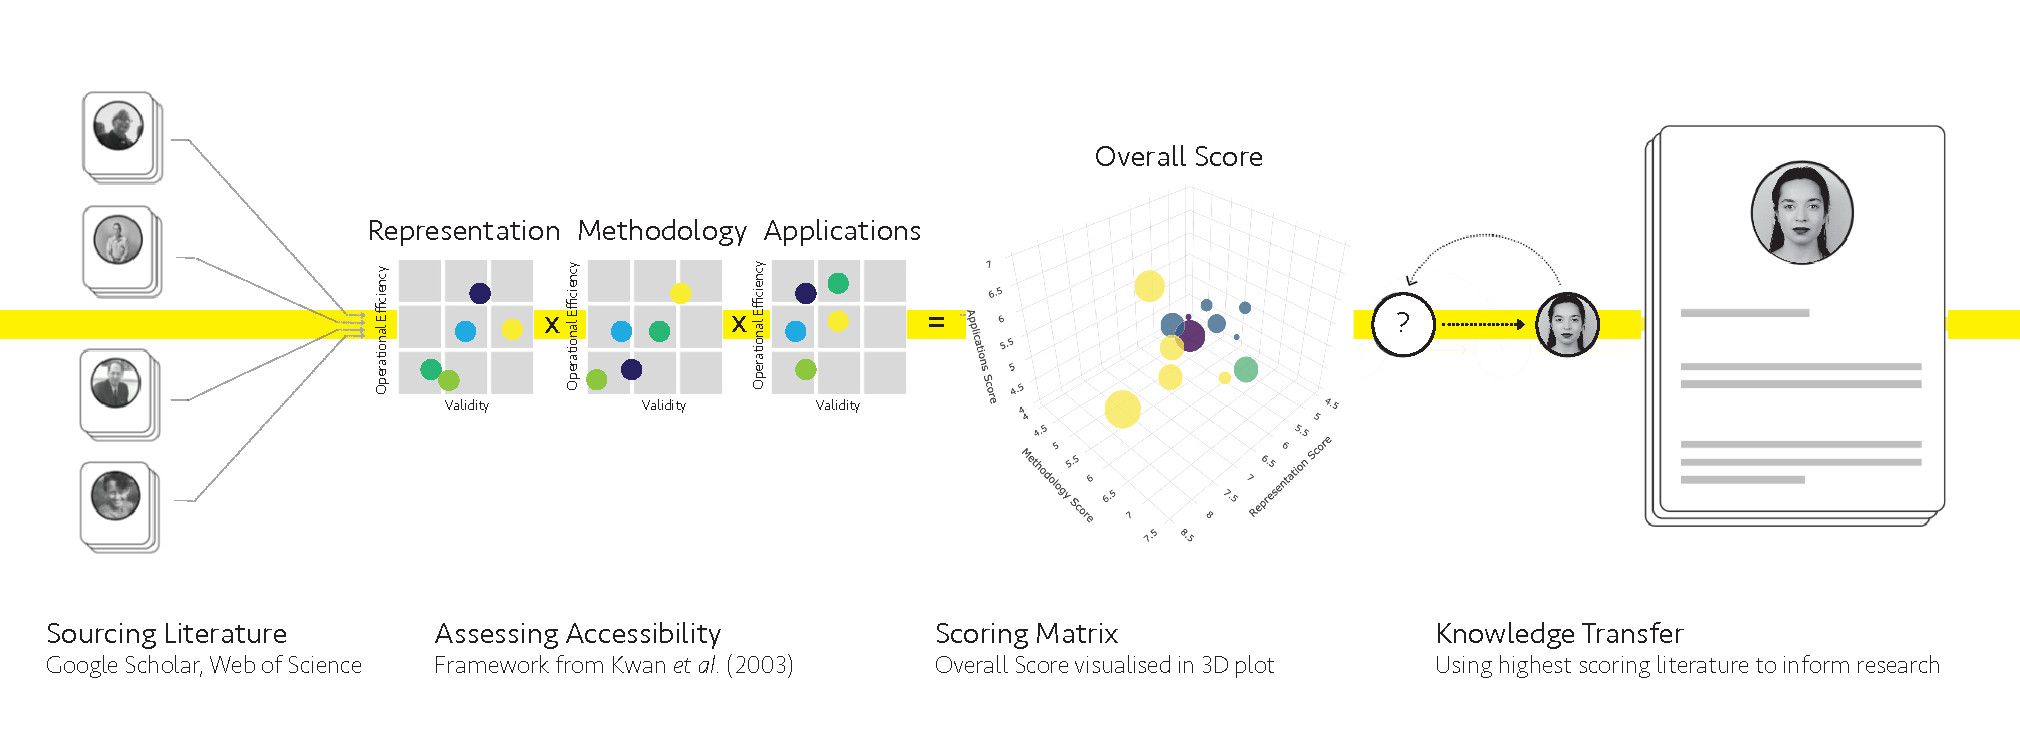
\includegraphics[width=1.2\textwidth]{Literature_review/Literature_Analysis.pdf}}
    \caption[Literature Analysis Methodology]{Process of analysing and evaluating literature on accessibility.} 
    \label{fig:Literature_Analysis}
\end{figure}

\subsection{Defining Accessibility}
The definition of accessibility previously depended on the context of its application. In early literature, accessibility was measured purely as a function of utility, defined as the likelihood of an individual choosing a particular destination based on the utility value of that choice compared to other perceivable choices (Bogue 1949). Since then, academics such as Hansen (1959) have measured accessibility geographically and argued that accessibility should be understood as a function of the potential opportunities for spatial interaction “adjusting for the ability and desire of people or firms to overcome spatial separation” (1959: 5). Although a seminal paper, Hansen’s argument narrows the definition of accessibility to employment and retail opportunities, perhaps showing a limited understanding of spatially distributed activities. In addition, Hansen's method removes spatial granularity by categorising land as inter-urban (between urban areas) and intra-urban (within urban areas), which fails to indicate the nuanced differences between rural, suburban and central city accessibility patterns. A more pragmatic understanding of accessibility has been introduced by Van Wee and Geurs (2011), who defined accessibility as “the extent to which land use and transport systems enable individuals to reach activities and destinations” (2011: 351). They argue that the definition of accessibility should combine location based and utility based theory, yet be computed with models using spatially granular data. I adopt this definition as a foundation to develop an approach that combines a location based measure of accessibility with a novel methodology, to analyse the neighbourhood characteristics that determine local access to employment opportunities.

\subsection{Assessing accessibility}
Although the components of accessibility are difficult to define, they are crucial to develop an understanding of the level of access individuals have to employment opportunities. I summarise the historical and contemporary approaches of measuring accessibility in figure \ref{fig:Literature_timeline_new}. The timeline shows that both the theoretical approach and modelling strategies evaluating accessibility change from spatial aggregations of accessibility (Hansen 1959) to individual, real-time measurements (Kim and Kwan 2019). 

\begin{figure}[H]
    \centering
    \makebox[\textwidth][c]{\includegraphics[width=1.2\textwidth]{Literature_review/Literature_timeline.pdf}}%
    \caption[Literature Timeline]{The notable academics and their key approaches to measuring accessibility from 1950 to 2019.} 
    \label{fig:Literature_timeline_new}
\end{figure}

The key literature can be categorised as two approaches; location based measures and person based measures. On the one hand, location based measures describe the relationship between accessibility and residential segregation, such as Glaeser \textit{et al}’s (2008) analysis of the suburbanisation of poverty, and lower rates of upward mobility for Hispanic and African Americans (Chetty \textit{et al.} 2014). On the other hand, person based measures of accessibility capture its gender differences (Kwan 1998: 191). Regardless of whether the literature reflects the spatial distribution of accessibility or individual accessibility, the academic field is developing an appetite for new methodologies using contemporary techniques and novel datasets (Chen \textit{et al.} 2016, de Bruijn \textit{et al.} 2018).

I develop a systematic literature review based on Kwan \textit{et al’s} (2003) framework which assesses the “simultaneous treatment of representation, methodology and application” (2003: 129). I adopt this evaluative structure in my analysis of accessibility to evaluate whether there is an accurate representation of accessibility, whether accessibility modelling is valid, and if there is a clear application of accessibility research. 

\subsection{Representation}
I will analyse representations in three respects, spatially aggregated accessibility, individual accessibility, and space-time representations of accessibility. I summarise these three representations of accessibility in terms of their operational efficiency (ability to simplify the representation of accessibility) and validity (accurate representation of accessibility) (figure \ref{fig:Representation}).

\begin{figure}[ht]
    \centering
    \includegraphics[width=0.99\textwidth]{Literature_review/Representation.pdf}
    \caption[Representation scatterplot]{Graph showing representation scores for each key piece of literature. The node colour indicates the type of accessibility indicator the literature uses (infrastructure based, location based, utility based and person based).} 
    \label{fig:Representation}
\end{figure}

\subsubsection{Representing Space}
Spatial accessibility can be analysed through a “zone-based, aggregate spatial framework (e.g. census tracts or block groups)” (Kwan \textit{et al.} 2002: 130). More broadly, representing the spatial distribution of accessibility illustrates the latent structure of the location of individuals in relation to the location of employment opportunities. An example of expressing accessibility spatially is Chetty \textit{et al.} (2014), who attribute accessibility to commuter zones, which are geographical aggregations representing local economies (USDA 2000). Chetty’s research uses large spatially aggregated datasets which rely on the assumption that processes determining the distribution of accessibility are only measurable at the regional level. Although it may seem intuitive to represent access to employment by commuter zones, this is problematic as accessibility can be a function of household level processes, such as car ownership and income. Furthermore, the geography of accessibility in American cities is changing, therefore it is difficult to define the appropriate spatial aggregation at which spatial patterns of accessibility exist. The pivotal issue with aggregating accessibility to geographic units is the modifiable areal unit problem (MAUP) defined as the geographic pattern of accessibility that occurs only due to the areal unit that the data is collected (Openshaw and Taylor 1979). Within accessibility research the MAUP is of serious methodological concern, and presents a fundamental challenge to spatial aggregations of accessibility.

\subsubsection{Representing Individuals}
Answering the literature’s lack of consensus on modifiable areal unit problem is the work of Mei-Po Kwan, who argues we should challenge the focus on place based measures of accessibility, and instead measure accessibility at the individual level. Kwan’s research shifts our understanding of the MAUP to acknowledge there are multiple uncertainties introduced when measuring accessibility using the concept of UGCoP (The Uncertain Geographic Context Problem). For example, Weber and Kwan (2003) argue that spatially aggregated measures of accessibility are no longer able to cope with the complex relationships between “urban form, mobility and individual accessibility” (2003: 341). Although new data collection methods allow accessibility to be measured at the individual level, arguably, Weber and Kwan overemphasise the individual as the sole determinant of access to spatially distributed activity. Adopting this stance is Manley (2006) and Jones \textit{et al.} (2018), who argue the social relationships regulating individual accessibility can only be observed “through the analysis of data at an aggregate level” (Manley 2006: 15). Responding to this, Kwan and Ren (2008) argue both geography and individual experience is represented by “space-time accessibility” (2008: 109).

\subsubsection{Representing Space and Time}
A space-time framework, originally developed by 
Hägerstrand (1970), attempts to measure the “behavioural possibilities of individuals” (Miller 1991: 287). A space-time framework suggests there are spatial and temporal limitations on individual accessibility, represented by the “space-time prism” (Miller 1991: 291). A space-time prism models individual activity participation at different locations throughout the day; an approach that values activity sequences rather than spatial aggregations of activity concentration. Recent representations of space-time accessibility include Kim and Kwan (2019), who illustrate that individuals living in the same residential location experience different exposure to congestion due to their “idiosyncratic activity-travel patterns” (2019: 15). The advent of “big spatiotemporal data” (Chen and Kwan 2018: 1), defined as data measured at an exceptionally granular level through space and time, allows researchers to represent space-time accessibility patterns more accurately. As this data becomes more available and computationally efficient to process, it is likely space-time representations will grow in importance in the accessibility literature.

\subsection{Methodology}
The methodologies for analysing accessibility are assessed in terms of their operational efficiency (model parsimony) and validity (the model’s incorporation of all significant predictors influencing accessibility) (figure \ref{fig:Methodologies}).

\begin{figure}[ht]
    \centering
    \includegraphics[width=0.99\textwidth]{Literature_review/Methodology.pdf}
    \caption[Methodology scatterplot]{Graph showing methodology scores for each key piece of literature.} 
    \label{fig:Methodologies}
\end{figure}

\subsubsection{Aggregated Modelling}
During the 20th century, aggregated modelling measured accessibility as distance to the Central Business District (CBD) from the areal unit the resident occupies (Harris and Ullinan 1945, Alonso 1964, Muth 1969). The assumption underlying this measurement of accessibility is that the further away from the economic centre a resident lives, the less accessibility they have to spatially distributed activities. Although geographic proximity to spatially distributed activities is in no sense the sole determinant of accessibility, there is a strong correlation between access and centrality, in particular when measuring accessibility at small travel times. However, this simplification of accessibility results in a crude understanding of actual locational attractiveness, and there has been a dramatic shift in the explanatory capacity of the urban form to be an “organising principle” of accessibility (Kwan and Weber 2003: 343). For example, the construction of freeways through large American cities reduced the place based advantage of living in central metropolitan areas. 

\subsubsection{Multilevel Modelling}
In transportation literature, multilevel analysis has heavily focussed on time-based accessibility to measure activity participation (Goulias 2002, Kwan \textit{et al.} 2003), because multilevel analysis already lends itself well to explicitly model the spatial dependency of accessibility outcomes. For example, Hong and Goodchild (2014) use a multilevel model (MLM) to specify the spatial and temporal structure of accessibility to infer the relationship between land use patterns and transport emissions in urban and suburban locations. The multilevel framework provides enough flexibility to analyse accessibility across space and through time in a two level model, with timestamps nested in spatial locations. Furthermore, multilevel modelling can account for both individual level accessibility within spatially aggregated units, as Weber and Kwan (2003) locate space-time accessibility values for individuals within neighbourhoods. Multilevel research offers a successful framework to model place based accessibility, but practitioners must specify the spatial or temporal structure of the data and cannot measure accessibility only at a single level.

\subsubsection{Machine Learning}
Although many geographers argue that the spatial level is where the fundamental relationships of accessibility are played out (Manley 2006, Jones \textit{et al.} 2018), multilevel modelling cannot account for dynamics that are only measurable at the individual level. Complementing this pivot away from place based measures of accessibility is the development of georeferenced activity-travel data and efficient GIS-based methodologies to analyse big datasets (Chen \textit{et al.} 2018). For example, Kim and Kwan (2019) collect real-time traffic congestion and activity-travel data of 250 individuals in Los Angeles to analyse exposure to congestion, and conclude that only individual activity trajectories can reveal the true variation in exposure to traffic congestion. An example of using big data to inform predictions is Li \textit{et al.} (2019), who develop a machine learning algorithm to predict the location of individuals and their likely future activity spaces. Both studies move dramatically away from theory-driven approaches like multilevel modelling, and instead apply data-driven approaches to analyse individual accessibility. However, there is little consensus on the cleaning, analysis and reporting of results for big data, and the literature needs to develop a peer-reviewed framework to standardise analysis.

\subsection{Applications}
After discussing the issues with multiple representations and methodological concerns of analysing accessibility, I assess the social and economic applications of measuring accessibility. This is evaluated in terms of their operational efficiency (ease at which the measurement of accessibility can be applied to urban and transportation planning) and validity (how meaningful the application is) (figure \ref{fig:Applications}).

\begin{figure}[ht]
    \centering
    \includegraphics[width=0.99\textwidth]{Literature_review/Applications.pdf}
    \caption[Application scatterplot]{Graph showing the application scores for each key piece of literature.} 
    \label{fig:Applications}
\end{figure}

\subsubsection{Accessibility as an economic indicator}
In 2012, although 23 percent of lower income residents lived in central urban locations, suburban poverty experienced a 139 percent increase between 2000-2012 (National Center for Law and Economic Justice 2014). These low income, suburban neighbourhoods face a compilation of challenges, such as high crime rate, poor health, low-performing schools and low job density, all of which are exacerbated by lacking transit options. Communities who experience low job accessibility are likely to earn a low wage, thus have reduced opportunities to achieve upward mobility (Kain 1968, Kasarda 1989, Wilson 1996). More recently, Chetty \textit{et al.} (2014) performed a correlation analysis on spatially aggregated accessibility data, showing that communities located in central city areas experience higher rates of upward mobility (\(R^2\) = 0.6). Furthermore, many lower income households who relocate to suburban neighbourhoods do so to raise children, increasing the rate of suburban childhood poverty. The 2009 National Household Travel Survey show that households with children tend to travel over twice the distance than households without children, thus, there is strong evidence suggesting suburban, low income families spend a higher proportion of their income on transportation expenses (FHWA 2014). Households spend 33 and 16 percent of their average annual expenditure on housing and transportation, and as both costs continue to rise, lower income families are likely to face an increased cost burden for even basic travel expenses (Bureau of Labor Statistics 2017). 

\subsubsection{Accessibility as a social indicator}
More recently, literature has focussed on the ethnic makeup of neighbourhoods and their location in American cities (Van Wee and Geurs 2011, Cort \textit{et al.} 2014). National statistics indicate that African American and Hispanic households are disproportionately represented in low income, suburban neighbourhoods, and these cost-sensitive ethnicity groups experienced poverty rates of 27 and 26 percent respectively, when the overall poverty rate is much lower at 14 percent (DeNavas-Walt \textit{et al.} 2012). Furthermore, Hispanics have the highest person and vehicle trips of all ethnic groups, and experience the lowest mobility and highest levels of poverty (FHWA 2014). Due to the residualisation of low income minority groups, the most recent National Household Travel Survey concludes it is essential for minorities have access to affordable and effective transportation options enabling them to access job opportunities. Nowhere is this more pertinent than in large American cities, as 44 percent of Hispanics live in the ten largest metropolises, and in Los Angeles the Hispanic population is 48 percent (FWHA 2014, U.S. Census Bureau 2012). Upward mobility is the ultimate goal of accessibility (Vickerman 1974), and therefore it is essential we consider the social and economic barriers to implement effective transportation policy.

\subsection{Evaluating the Research Gap}
After taking the average scores for the representation, methodology and application of accessibility for the key literature, I visualise the combined score on a 3D interactive plot\footnote{Interactive version: \url{https://github.com/ChristinaLast/Equity-Accessibility-Los-Angeles}} (figure \ref{fig:Literature_matrix}). The plot represents the literature’s average score for all three sections with the node size scaled by their standard deviation. Notably, there is a strong linear relationship between all three framework sections with person based and location based measures of accessibility performing highly. Location based measures of accessibility show a small standard deviation (suggesting high performance in all categories), which led me to adopt a location based measure of accessibility. However, what both person and location based measures fail to achieve is an accurate representation and useful application of accessibility. To narrow this research gap, I develop a simple methodology employing a novel machine learning technique to accurately represent accessibility patterning in Los Angeles.\begin{figure}[ht]
    \centering
    \makebox[\textwidth][c]{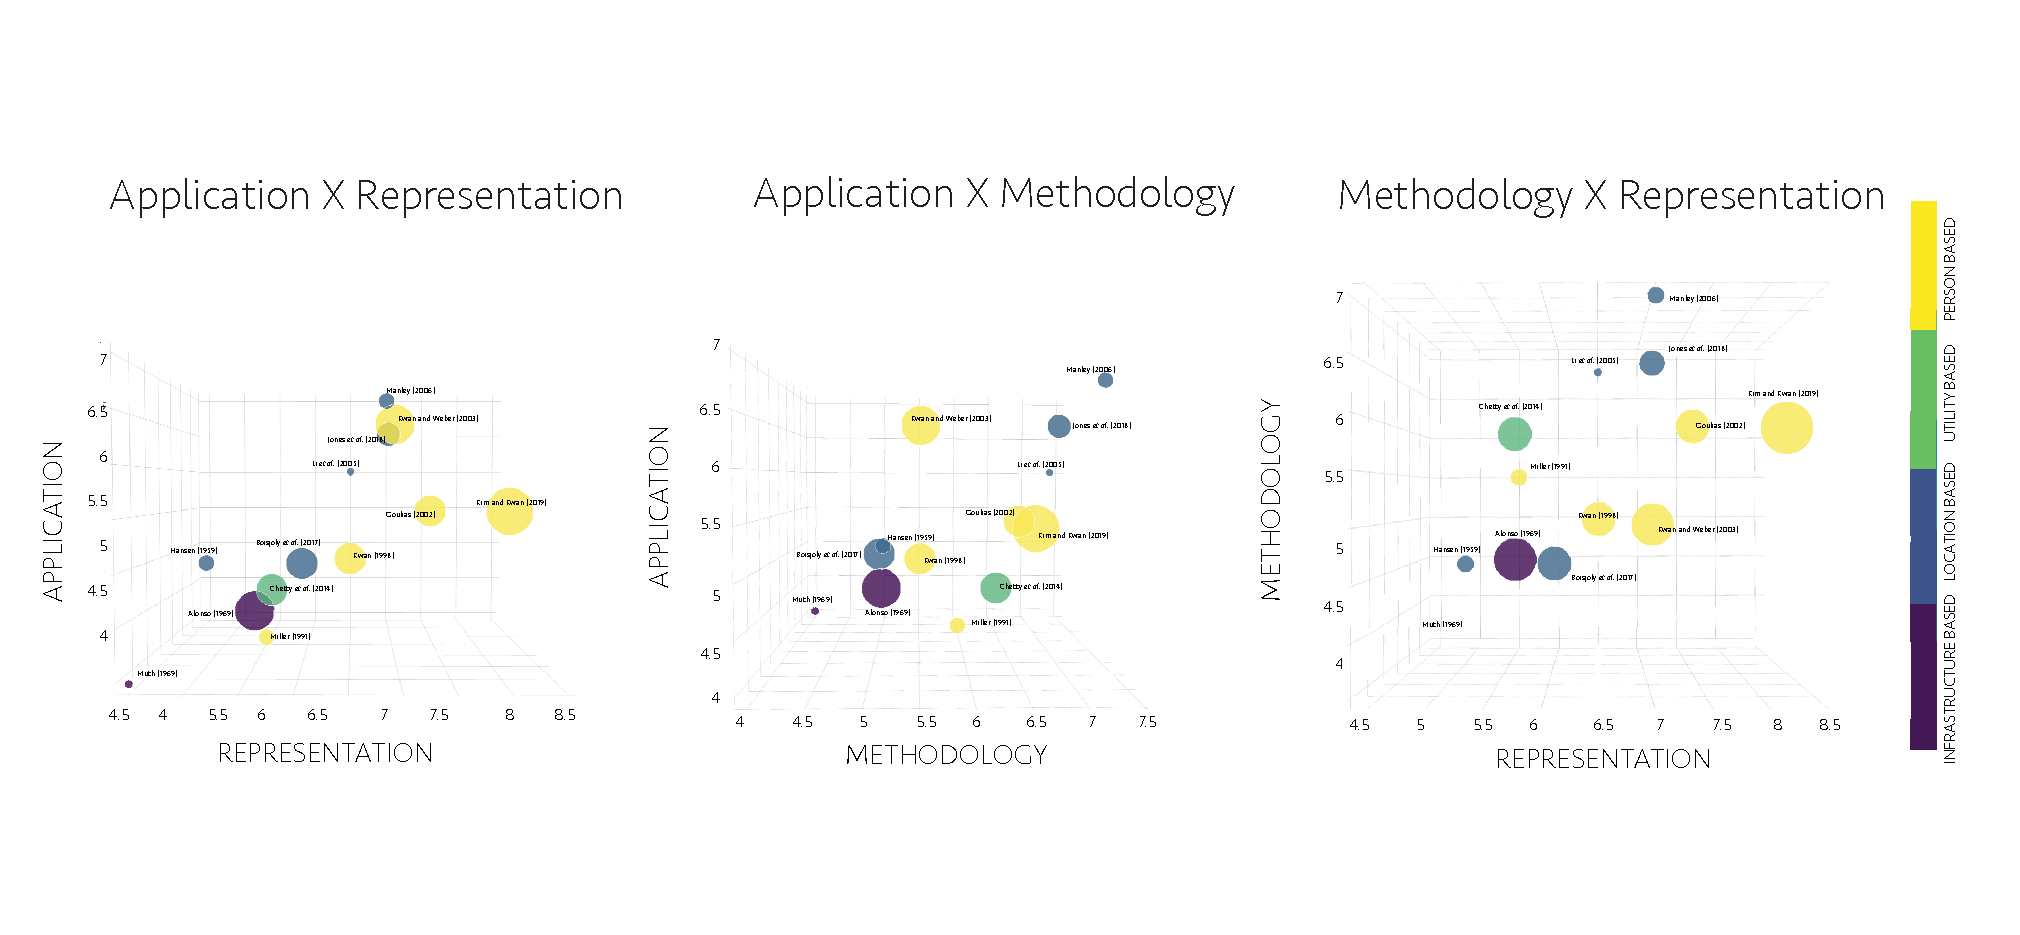
\includegraphics[width=1.3\textwidth]{Literature_review/Literature_matrix.pdf}}
    \caption[Combined 3D scatterplot]{A 3D scatterplot showing the combined scores for the accessibility literature, showing three axis views of (a) application and representation, (b) application and methodology and (c) representation and methodology, with each literature node scaled by their standard deviation.} 
    \label{fig:Literature_matrix}
\end{figure}

\subsection{Narrowing the Research Gap}
The recent development of spatially granular accessibility data provides a rich evidence base to test the relationship between ethnicity and their household and transportation expenditure burdens. Additionally, there has been limited research comparing the predictive accuracy of multilevel modelling (MLM) and machine learning methods (Feng and Jones 2015), and none developing a clear methodology for analysis. Furthermore, there is no agreement on whether larger or smaller training data is more suitable for model training. Finally, there has been slow adoption of novel modelling approaches that account for the “spatial spillover effects” of low neighbourhood equity in the transportation literature.

To address this gap, I combine data from the Center for Neighborhood Technology (2017), the US Census Bureau (2010) and Chen \textit{et al's} (2011) Opportunity-Based Accessibility indicators to analyse the variety of social, environmental and economic parameters influencing accessibility patterns. To improve the previous approaches to modelling accessibility, I build on Feng and Jones’ (2015) comparison of MLM and ANN by incorporating spatial spillover effects using an SLX model (Vega and Elhorst 2015). Introducing a spatial weights matrix into the multilevel model and the neural network evaluates the spatial spillover of low equity neighbourhoods while maintaining model parsimony. The results contribute important findings on the location of ethnic communities with low accessibility to the Metro 2028 Vision Plan and the Los Angeles Sustainability Plan (Petersen \textit{et al.} 2018), both recent initiatives to improve access to high quality mobility options in Los Angeles County. Overall, this research aims to push our current ability to model location based accessibility with existing techniques, by adopting machine-learning modelling approaches that account for spatial effects. 

\subsection{Research Questions}
Having motivated the research gap and modelling strategy, the following list presents the specific research foci I seek to answer: 

\begin{itemize}
\begin{enumerate}
\item \label{itm:first} To what extent do household and transportation costs as a percentage of total income matter in determining accessibility to employment opportunities?
\item \label{itm:second} Is there evidence of spatial spillovers that explain differences in accessibility to employment opportunities?
\item \label{itm:third} What is the relative effect of being a Hispanic or African American in determining the level of accessibility to employment opportunities?
\end{enumerate}
\end{itemize} 


\pagebreak
\section{Data and Methodology}
This paper compares two advanced modelling approaches, artificial neural networks (ANN) and multilevel modelling (MLM) to model spatial patterns expenditure burdens faced by different ethnic groups and their effect on accessibility to employment in Los Angeles County. An artificial neural network is a modelling procedure that imitates the connections between biological neural networks, whereas a multilevel model is defined by the organisation of model parameters into different hierarchical structures. To account for the structural spillover effects of spatial units, I introduce a spatial weights matrix. I evaluate the model performance by mapping the residuals and the error values from the accessibility predictions. 

\subsection{Data overview and Setting}
This study selects Los Angeles County as the study area there are a diverse range of transportation options and a mixture of urban and rural land use incorporating both affluent suburbs and inner city areas. The 2009 National Household Travel Survey shows that in Los Angeles, an individual’s travel radius is affected by their level of income and ethnicity. For example, individuals earning over \$100,000 have a 23 mile travel radius, whereas for individuals below the poverty line this is only 11 miles (FWHA 2014). According to 2010 Census data, 53 percent of Hispanic and 25 percent of African American households are at or below the poverty line in Los Angeles County, compared to a county average of 15 percent. Compounding the effects of this limited travel radius, Los Angeles County also accounts for 481 million unlinked passenger trips, the third highest in the US, showing how restrictive travel choice can be for ethnic minorities in impoverished neighbourhoods. 

To explore the relationship between equity and accessibility for both Hispanics and African Americans in Los Angeles County, this study uses equity and ethnicity data to predict local accessibility. The null model tests the hypothesis that there is no difference in local accessibility in Los Angeles (measured as the number of jobs accessible by private vehicle over 10 minutes of travel time on the road network), using a multilevel model framework (Table \ref{tab:table1}). Model 1 introduces household and transportation expenditure as a percentage of income, to predict accessibility in Los Angeles County. To test whether there are “spatial spillover effects” of experiencing a similar level of equity burden as nearby neighbourhoods, I introduce a spatial lag of household and transportation expenditure in Model 2. In Model 3, I test if there is a relative effect of being in a high percentage African American or Hispanic neighbourhood on accessibility. To do this, I introduce the percentage of tract who are Hispanic and African American alongside household and transportation expenditure to predict local accessibility.

\begin{table}[H]
 \singlespacing 
 \centering
 \small
 \begin{tabular}{p{1.6cm}p{3cm}p{5cm}p{3.5cm}} 
 \toprule
 Model & Hypothesis & Equation & Variables Added \\ [0.5ex] 
 \hline
 Null Model & 
 There is no difference in accessibility between blocks, block groups and tracts. & 
 \[y_{ijk} = \beta x_{ijk} + \epsilon_{ijk}\] & The number of jobs accessible by private vehicle over 10 minutes on the road network. \[(\beta x_{ijk})\] \\ 
 Model 1 & 
 The percentage of income spent on household and transportation costs has an effect on accessibility to employment opportunities. & 
 \[y_{ijk} = \alpha_{jk} + \beta x_{ijk} + \epsilon_{ijk}\] Where \[\alpha_{jk} = \theta z_{jk} + \eta_k + \upsilon\] & 
 Percentage of income spent on household and transportation costs. \[(\alpha_{jk})\] \\
 Model 2 & 
 The spillover effect of household and transportation costs from neighbouring  geographic units has an effect on accessibility to employment opportunities. & \[y_{ijk} = \alpha_{jk} + W_{jk}\alpha\theta + \beta x_{ijk} + \epsilon_{ijk}\] Where \[W_{jk} =  \frac{1}{d^\gamma_{jk}}\] & 
 The percentage of income spent on household and transportation costs.  \[(\alpha_{jk})\] 
 The spatially lagged value for the percentage of income spent on household and transportation costs. \[(W_{jk})\] \\
 Model 3 & 
 There is a relative effect of being in high percentage African American or Hispanic neighbourhood on accessibility to employment opportunities. & 
 \[y_{ijk} = \alpha_{jk} + \eta_k + \tau + \beta x_{ijk} + \epsilon_{ijk}\] Where \[\eta_k =  \Gamma\xi_k + \nu\] \[\tau_k =  \Upsilon\omega_k + \upsilon\] & 
 Percentage of income spent on household and transportation costs \[(\alpha_{jk})\]
 The percentage of a census tract who are Hispanic. \[(\eta_k)\]
 The percentage of census tract who are African American. \[(\tau_k)\] \\
 \bottomrule
 \end{tabular}
 \caption[Table 1]{The hypothesis equation and description of the variables sequentially introduced into each model.}
 \label{tab:table1} 
\end{table}

\subsection{Variables}
\subsubsection{Response Variable}
I make use of block level accessibility data produced from the Southern California Association of Governments (2001), who use a “second-by-second and parcel-by-parcel modeling and simulation” (Chen \textit{et al.} 2011: 58). There is accessibility data for 16,470 blocks, indicating high accessibility (over 100,000 jobs) in Downtown Los Angeles, and under 62,000 in suburban locations, particularly in north and east Los Angeles County (Figure \ref{fig:Tot_r_10}). This data is referred to as 'true accessibility' throughout the study, and is used to draw conclusions on the accuracy of the MLM and ANN predictions. To construct this accessibility index, Chen \textit{et al.} (2011) develop a methodology using GIS to measure accessibility by cumulatively counting the instances of activities within travel time thresholds (10, 20, and 50 minutes) from each census block centroid. In this study I am interested in local accessibility, therefore I select total accessibility after 10 minutes of travel on the road network, and use the 11am-12pm low period to measure ambient accessibility. Over 25 percent of trips were completed in 7 minutes in the 2001 SCAG Regional Travel Survey, giving a good representation of local access (Chen \textit{et al.} 2011: 63). I acknowledge as this data is modelled rather than directly measured, so there may be inconsistencies between the accessibility data and actual accessibility.

\begin{figure}[ht]
    \centering
    \includegraphics[width=0.99\textwidth]{Data_methodology/Tot_r_10.pdf}
    \caption[Total local Accessibility]{The distribution of total accessibility by private transportation after 10 minutes of travel time.} 
    \label{fig:Tot_r_10}
\end{figure}

\subsubsection{Equity Predictors}
An important distinction between equity and equality is made by Van Wee and Geurs (2011: 351) who argue access to jobs can be unequal, however only the systematic exclusion of a certain population makes the distribution of accessibility inequitable. To measure equity, I include the percentage of income spent on Housing and Transportation costs (HTI) in the model specification. The HTI data is collected at the block group level and is constructed from data measuring “auto ownership, auto use and transit use” (Center for Neighbourhood Technology 2017: 6). Residents in Downtown Los Angeles spend around 10 percent of income on household and transportation, whereas areas in suburban Los Angeles spend between 60 to 80 percent of income on HTI costs (Figure \ref{fig:ht_ami}). The distribution of both accessibility and HTI is similar, reflecting the significant influence transportation expenditure has on accessibility.

\begin{figure}[ht]
    \centering
    \includegraphics[width=0.99\textwidth]{Data_methodology/ht_ami.pdf}
    \caption[Household and Transportation costs]{The distribution of household and transportation costs (\% of income).} 
    \label{fig:ht_ami}
\end{figure}

\subsubsection{Ethnicity Predictors}
Households that report a high percentage of income spent on household and transportation costs are disproportionately represented by African Americans and Hispanics (FWHA 2014). In the USA, these ethnic groups experience limited vehicle availability and less affordable transport options. To measure whether there is an inequitable distribution of access to jobs for different ethnicities in Los Angeles County, I introduce the percentage of the census tract population who are Hispanic or African American. The majority of census tracts in south central Los Angeles are over 50 percent African American (Figure \ref{fig:Black_African_American}a). In contrast, figure \ref{fig:Black_African_American}b shows Hispanic populations are more spatially distributed, but there are many tracts in east Los Angeles with over 80 percent Hispanic population. 

\begin{figure}[H]
    \includegraphics[width=0.49\textwidth]{Data_methodology/Black_African_American.pdf}
    \includegraphics[width=0.49\textwidth]{Data_methodology/Hispanic.pdf}
    \caption[African Americans and Hispanics]{The distribution of (a) African American and (b) Hispanic population in Los Angeles County.}
    \label{fig:Black_African_American}
\end{figure}

\subsubsection{Spatial Weights Matrix}
Dong \textit{et al.} (2019) argue that “geography exists both ‘vertically'... and ‘horizontally’” in the sense that geographic spillover effects between locally clustered areal units exist (2019: 119). Previously, standard econometric techniques have difficulty parameterising the “spatial spillover effects” of a neighbouring geographic unit. Vega and Elhorst (2015) introduce the SLX model to incorporate spatial effects into advanced modelling procedures, allowing changes to explanatory variables to impact neighbouring geographic units. I incorporate the SLX model to measure the “spatial spillover effects” of experiencing a similar level of equity burden as near neighbourhoods. The logic underpinning this is the more a block spends on household and transport costs, the more likely neighbouring blocks will experience an increase in household and transportation costs, through rent increases or fare increases on transportation. The SLX is beneficial as it measures the magnitude and significance of spillovers in a flexible and parsimonious specification of the spatial weights. 

\subsection{Methodology Overview}
\subsubsection{Multilevel Model}
As indicated in Chapter 2, multilevel modelling (MLM) is an invaluable approach to answering research questions with hierarchically organised data. More specifically, multilevel models analyse nested variability as a function of explanatory variables. Two important advantages of MLM is first, its flexibility in controlling for characteristics at multiple layers of analysis, and second, its ability to borrow strength from other data points. 

To analyse accessibility in a multilevel model, I first visually describe accessibility and organise the data into a nested data structure (Figure \ref{fig:MLM_diagram}). After replicating this structure in all model specifications (Technical Appendix, Section 8.1) I incorporate an additional parameter to answer each research question. Then I map the model residuals and model errors. 

\begin{figure}[ht]
    \centering
    \makebox[\textwidth][c]{\includegraphics[width=1.2\textwidth]{Methodology/MLM_diagram.pdf}}
    \caption[Multilevel modelling process]{Figure showing the process of the multilevel analysis.} 
    \label{fig:MLM_diagram}
\end{figure}

\paragraph{Model Specification}
All multilevel models were specified in Pystan and fit using Hamiltonian Monte Carlo. To structure a multilevel framework for a nested three-level model, I specify the between-block equation, the between-block group equation, and the between-tract equation. The combined three level model is represented at the block level by: 
\begin{equation} \label{eq1}
\hat{y} \sim N_N(\alpha + \beta x, 	\sigma^2_\epsilon)
\end{equation}
At the block group level:   
\begin{equation} \label{eq2}
\hat{\alpha} \sim N_J(Z \theta + \eta, \sigma^2_\theta)
\end{equation}
At the tract level:
\begin{equation} \label{eq3}
\hat{\eta} \sim N_K(P\zeta, \sigma^2_\zeta
\end{equation}
And the error terms are given such that: 
\[\hat{\epsilon} \sim N_N(0, \sigma^2_\epsilon);\] 
\[\hat{\theta} \sim N_J(0, \sigma^2_\theta);\]
\[\hat{\zeta} \sim N_K(0, \sigma^2_\zeta);\] 

The model structure includes $y$; the estimated total accessibility after 10 minutes of travel time (TOTR10) at the block level $N$, $J$ and $K$ are block group and tract level indicators. $\eta$ is the tract level influence on accessibility, and $\alpha$ the block group level influence. $N$ is number of blocks in $J$ block groups and $K$ tracts and is constrained to be positive. $\beta$, $Z$ and $P$ correspond to the vectors of the regression coefficients I will estimate. The terms $\epsilon$, $\theta$ and $\zeta$ are the residuals at the block, block group and tract levels, assumed to follow a normal distribution corresponding to the variance in $\sigma^2_\epsilon$, $\sigma^2_\theta$ and $\sigma^2_\zeta$.

\subsubsection{Artificial Neural Network}
Artificial neural networks (ANN) are a form of artificial intelligence designed to simulate biological neurons to process information, such as data classification and pattern recognition.  To analyse accessibility data using ANN, I build a sequential, feed-forward neural network using two dense layers and visualise the residuals (Figure \ref{fig:ANN_diagram}). To analyse the results, I map the model residuals and error to identify significantly high or low predictions of access to employment. 

\begin{figure}[ht]
    \centering
    \makebox[\textwidth][c]{\includegraphics[width=1.2\textwidth]{Methodology/ANN_diagram.pdf}}
    \caption[Artificial Neural Network analysis process]{Figure showing the process of building and analysing the artificial neural network.} 
    \label{fig:ANN_diagram}
\end{figure}

\paragraph{Model Specification}
An artificial neural network is constructed by connecting processing nodes to create hidden network layers between an input and output layer. Each layer is made of neurons, and the strength of the connection between the neurons is a function of a set of weights. The weight $w_{ij}$ depends only on information locally available: the state properties of the neurons $i$ and $j$. For example, if neurons $i$ and $j$ are in the same state $w_{ij}$ and will increase, and if they are different $w_{ij}$ will decrease (Coolen 1998). This definition can be written as:
\[S_i = S_j: \uparrow w_{ij}\]
\[S_i \neq S_j: \downarrow w_{ij}\]
\[w_{ij} \rightarrow w_{ij} + S_i S_j\]

\subsection{Testing Predictions}
I use Bayesian inference to quantify the uncertainty in my predictions of accessibility from the probability distribution of prior estimates. However, as it is impractical to calculate the probability distributions at each iteration of the model, I take advantage of the stochastic sampling method Markov Chain Monte Carlo (MCMC) using the probabilistic programming language Stan\footnote{\url{https://github.com/stan-dev}}. Due to the introduction of variance in the regression slopes for all predictor variables, MCMC estimates are beneficial as the predictions “yield exact inferences in situations where maximum likelihood only provide approximations” (Fielding and Goldstein 2006: 46). 

To check for robustness in the multilevel model I evaluate a series of trace plots for each parameter introduced into the model. Uncertainty during Bayesian estimation is captured in the spread of the posteriors described in each traceplot. In addition to the traceplots, I evaluate the success of the multilevel model and the artificial neural network in terms of their goodness of fit (measured by $R^2$), predictive accuracy, measured as the Mean Absolute Error/Mean Absolute Percentage Error (MAE/MAPE) and explanatory capacity. To evaluate each model’s explanatory capacity, I analyse the residual plots and error plots for each modelling technique. 

\subsection{Software}
All data cleaning, imputation, and visualisation was conducted in Python 3.7\footnote{\url{https://www.python.org/downloads/release/python-370}}. I use PyStan\footnote{\url{https://pystan.readthedocs.io/en/latest/}} to build and run the multilevel model, and Tensorflow\footnote{\url{https://github.com/tensorflow/tensorflow}} to build the neural network. PyStan provides a Python interface to Stan, a package for Bayesian inference and sampling strategy using Hamiltonian Monte Carlo estimation. Stan is more efficient in high dimensional problems where there are a large number of predictors to infer. This lends itself well to my study, where there is over 29,000 rows of data. 

\pagebreak
\section{Results}
This section compares the results of a multilevel model (MLM) and an artificial neural network (ANN) using the aforementioned research questions (Question \ref{itm:first}, \ref{itm:second} and \ref{itm:third}). I evaluate the biases in the MLM and ANN by mapping clusters of predicted accessibility that are significantly different from the 'true' accessibility values (Chen \textit{et al.} 2009).
\subsection{Descriptive Statistics}
I describe the variables included in the study in Table \ref{tab:table2}. The full model for both the artificial neural network and multilevel model contains three predictors measured at the block group and tract level.

\begin{center}
\singlespacing
\begin{table}
\caption[Table 2] {\label{tab:table2} Descriptive statistics for all variables introduced into the models.} 
 \begin{tabular}{p{3cm}p{1.6cm}p{2.5cm}p{5cm}}
 \toprule
 Variable & Type & Descriptive statistics & Unit of Measurement \\ [0.5ex] 
 \hline Structural Variables & & & \\
 [0.5ex] 
 \hline
 Blocks &  & 16470 blocks & A unique identifier for each of the 16470 blocks \\ 
 Block groups &  & 3221 block groups & A unique identifier for each of the 3221 block groups \\
 Tracts &  & 1306 tracts & A unique identifier for each of the 1306 tracts \\ \\
 \hline
 Dependent Variables &  &  &  \\
 \hline
 Total Accessibility & Continuous & Min = 169 & Accessibility indicators are con- \\ 
 & & Max = 324814 &  structed by Chen \textit{et al.} (2016), and \\
 & & Average = 102862 & are calculated using an activity- \\
 & & SD = 57227 & based travel demand model by the Southern California Association of Governments. \\
 & & &  \\ \hline
 Predictor Variables &  &  &  \\
 \hline
 Household and & Continuous & Min = 17 &  The percentage of income spent on \\ 
 Transportation && Max = 100 &
 Household and Transport costs are \\
 Costs (as a && Average = 57 & constructed from a combination of \\ 
 percentage of & & SD = 14 & “auto ownership, auto use and \\
 income) & & & transit use” data (Center for Neighbourhood Technology 2017: 6) \\ \\ \hline
 Percentage of tract & Continuous & Min = 0 & The percentage of Hispanic is \\
 that are Hispanic & & Max = 100 & calculated from the total tract\\
 & & Average = 56 & population who are Hispanic \\
 & & SD  = 28 & divided by the total tract population.\\ \\
 \hline
 Percentage of tract & Continuous & Min = 0 & The percentage of African \\
 who are African  & & Max = 83 & American is calculated from the  \\
 American & & Average = 9 & total tract population who are \\
 & & SD = 15 & African American divided by the total tract population.\\
 \bottomrule
\end{tabular}
\end{table}
\end{center}

\doublespacing
\subsection{Performance Measures}
I adopt Feng and Jones' (2015) analysis framework to compare the goodness of fit, predictive accuracy and the explanatory power of the multilevel model and artificial neural network ({Table \ref{tab:table3}}). After evaluating the model fit, I discuss the predictor variables most influential on accessibility, introducing their coefficients and associated variability. 
\begin{center}
\begin{table}
\caption[Table 3] {\label{tab:table3} Table comparing the goodness of fit and accuracy measurements for the MLM and ANN using Mean Absolute error (MAE), Mean Absolute Percentage Error (MAPE) and $R^2$.} 
\begin{tabular}{p{2cm}p{1.6cm}p{1.2cm}p{0.9cm}p{1.2cm}p{1.6cm}p{1.2cm}p{0.9cm}}
 \toprule
MLM & \multicolumn{3}{c}{} & ANN & \multicolumn{4}{c}{} \\ \cline{2-4} \cline{6-8} 
        &  MAE  & MAPE & $R^2$        &             
	&  MAE  & MAPE & $R^2$                                                  \\    \hline
 Null Model   &  102861      &  99.9  &  0.1   &             &            &         &          \\     
 Model 1       &  5917.20     &  8.05  &  0.97  &  Model 1  &  33263.50  &  45.2   &   0.39   \\     
 Model 2       &  100868.86   &  97.76 &  0.1   &  Model 2  &  33445.33  &  46.75  &   0.35   \\
 Model 3       &  79914.64    &  76.90 &  0.15  &  Model 3  &  31794.47  &  43.76  &   0.42   \\
 \bottomrule
\end{tabular}
\end{table}

\end{center}
\subsubsection{Goodness of Fit}
A comparison of goodness of fit is presented in Table \ref{tab:table3}. A higher $R^2$ value indicates the model is more confident that the predicted accessibility is similar to the ‘true value’ of accessibility. The goodness of fit for the MLM does not improve because most of the variation in accessibility can only be explained by block level latent effects, therefore, the introduction of higher level (block group and tract level predictor variables) does not significantly explain the variation in block level accessibility. Alternatively, The $R^2$ value for ANN decreases from Model 1 to Model 2, yet increases in Model 3 when ethnicity parameters are introduced. The ANN results may show a reduction in goodness of fit when additional parameters are added to the model because there are too few neurons (4,160 and 65 neurons in two densely connected layers) which can restrict the representation the network learns, causing underfitting. 

\subsubsection{Predictive Accuracy}
Accuracy comparisons between the MLM and the ANN are summarised in Table \ref{tab:table3}. In one instance, the MLM shows high predictive accuracy in Model 1, as the mean absolute percentage error (MAPE) for MLM is reduced from 99 percent to 8 percent, however this increases in Model 2 when the SLX model is introduced (as the MAPE increases to 97 percent). In the other instance, the ANN improves gradually, reducing from 45 percent to 43 percent in Model 3. Other than Model 2, ANN remains the best performer in each scenario with an average error of 136,566 jobs. This demonstrates the capacity for ANN to extrapolate relationships from a small training dataset, even when access to jobs is non-normally distributed across Los Angeles County.

\subsubsection{Explanatory Capacity}
In the following sections I evaluate the explanatory capacity of each model specification, by visualising the residual errors from each model specification in comparison to the actual distribution of accessibility (TOTR10). I calculate the residual error by subtracting the accessibility prediction from the 'true value' of accessibility. To identify clusters of inaccurate predictions from the MLM and ANN I compute local error clusters from the predicted accessibility values, using a queen contiguity function. For any isolated predictions (where queen contiguity cannot identify neighbouring blocks) I use the k-nearest neighbours algorithm to complete a matrix of predicted error values and their spatial lag. Using a local Moran's \texitit{I} clustering algorithm (Section 8.2, Technical Appendix), I obtain the local clusters of predicted accessibility that are significantly different from their 'true value', and visualise them using the classifications; hot spot, cold spot, doughnut, diamond and no significance. The maps simultaneously compare both errors from the MLM and ANN predictions with the 'true values' of accessibility.

\subsection{Null Model}
I specify the null model using a multilevel framework. In the multilevel model, the specification exposes all blocks to varying levels of accessibility. The average block has access to 24.77 jobs, however the between-block variance is 117,700. This suggests there is unaccounted variability between blocks in this model specification, thus confounding variables need to be modelled to explain block-level variation. The between block group variability is 1.49, substantially smaller than the block level variance, and variation explained at the tract level is almost 0 (Figure \ref{fig:Fit_null_robust}). Figure \ref{fig:Model_null_multilevel} shows the null model does not capture the spatial concentration of jobs in Downtown Los Angeles. 

\begin{figure}[H]
    \centering
    \makebox[\textwidth][c]{\includegraphics[width=1.3\textwidth]{Results/Fit_null_robust.pdf}}
    \caption[Null Model Trace and Posterior plots]{Trace and distribution plot for (a) block group intercepts; (b) tract intercepts, and (c) block group level variance.} 
    \label{fig:Fit_null_robust}
\end{figure}

\begin{figure}[H]
    \centering
    \includegraphics[width=0.99\textwidth]{Results/Model_null_multilevel.pdf}
    \caption[Null Model predictions]{Predictions for local Accessibility (TOTR10) from the Null Model.} 
    \label{fig:Model_null_multilevel}
\end{figure}

\subsection{To what extent do household and transportation costs as a percentage of total income matter in determining accessibility to employment opportunities?}
Given my interest in exploring the relationship between equity and accessibility, Model 1 introduces the percentage of income spent on household and transportation costs (HTI) as  block group level parameter. To check for uncertainty, I plot the potential regression line, as well as the trace and posterior distributions (Figure \ref{fig:Fit_1_robust}a). The plots of posterior distributions show the model estimates are close the modes of our distributions (Figure \ref{fig:Fit_1_robust} b, c, d and e) and comfortably within the 95 percent confidence intervals. There is some bias between the peaks of the posteriors and the model estimates, which is a result of noise in the data. 		

\begin{figure}[H]
    \centering
    \makebox[\textwidth][c]{\includegraphics[width=1.3\textwidth]{Results/Fit_1_robust.pdf}}
    \caption[Model 1 Trace and Posterior plots]{Regression plot for (a) Household and transport costs (HTI) and Accessibility (TOTR10), the trace and distribution plot for HTI intercept (b), for HTI slope (c), for the block group intercepts (d), the trace and posterior for the log (e).} 
    \label{fig:Fit_1_robust}
\end{figure}
In the MLM the coefficient for household and transportation costs is 11.4 percent of income, which can be interpreted as, for every 1 percent increase in household and transportation costs accessibility decreases by 11.4 jobs. The between-block variance shrunk from 117,700 to 8,890 jobs, suggesting the inclusion of HTI costs reduces block-level uncertainty. However, the block group variability only slightly increases to 2.66 and tract level variation increases to 1.86, which fails to sufficiently explain accessibility at both neighbourhood levels.  Comparatively, the specification of the artificial neural network regresses HTI costs on accessibility. The average number of jobs accessible across all blocks is 103,178 jobs, however, due to the inability to partition variance at different levels, the ANN estimates block level variation in accessibility to be 35,691 (Table \ref{tab:table6} , Model 1), larger than the multilevel model prediction (Table \ref{tab:table4}). Upon visual inspection, the multilevel model accurately captures the degradation of accessibility in suburban locations, as eastern Los Angeles County there are as few as 4,000 locally accessible jobs (Figure \ref{fig:Model_1_multilevel}a). Although the neural network captures the spatial pattern of accessibility, explaining 39 percent of its spatial variation, the predictions become negative for suburban locations in north and east and south central Los Angeles (Figure \ref{fig:Model_1_multilevel}b). 

\begin{figure}[H]
    \includegraphics[width=0.49\textwidth]{Results/Model_1_multilevel.pdf}
    \includegraphics[width=0.49\textwidth]{Results/ANN_Model_1.pdf}
    \caption[Model 1 predictions]{Model 1 predictions for MLM (a) and ANN (b) and a scatterplot to show the residual distribution. } 
    \label{fig:Model_1_multilevel}
\end{figure}

Figure \ref{fig:Error_1_MLM_ANN} overlays the errors for the multilevel model and the artificial neural network. It shows that both modelling procedures significantly under predict the accessibility in eastern Los Angeles County  shown by the green error results (estimating under 95,000 jobs for the lowest 2.5 percent of blocks), and both MLM and ANN over predict some block level accessibility in Downtown Los Angeles shown by the yellow blocks, (estimating over 200,000 jobs) due to the right-skewed distribution of accessibility.  

\begin{figure}[H]
    \centering
    \includegraphics[width=0.99\textwidth]{Error/Error_1_MLM_ANN.pdf}
    \caption[Model 1 error]{The error from Model 1 for the MLM and ANN.} 
    \label{fig:Error_1_MLM_ANN}
\end{figure}

\subsection{Is there evidence of spatial spillovers that explain differences in accessibility to employment opportunities?} 
Model 2 incorporates the spatial lag of household and transportation costs to account for the spatial spillover effects of household and transportation costs. Put simply, the higher the proportion of income a census block spends on household and transportation, the more likely this will affect neighbouring census blocks, through rent increases or transportation fare increases. Analysing the uncertainty from figure \ref{fig:Fit_2_robust}c shows that the block-level variation is close to the mode of the distribution, and comfortably within the 95 percent confidence intervals. However, figure \ref{fig:Fit_2_robust}d shows the Markov chains at the block group level struggle to converge, suggesting HTI costs and the spatial lag of HTI are perfectly collinear at the block group level, and therefore are not separately identifiable within the model predictions.

\begin{figure}[H]
    \centering
    \makebox[\textwidth][c]{\includegraphics[width=1.3\textwidth]{Results/Fit_2_robust.pdf}}
    \caption[Model 2 Trace and Posterior plots]{Regression plots showing the relationship between (a) household and transportation costs (HTI) and Accessibility and (b) the spatial lag of HTI and Accessibility. The  trace and distribution plot for (c) the block level variance and (d) block group level variance.} 
    \label{fig:Fit_2_robust}
\end{figure}

The coefficient for HTI costs decreases to 1.2, suggesting for every 1 percent increase in household and transport costs, job accessibility increases by 1.2 jobs. Additionally, the coefficient associated with the inclusion of spatially lagged HTI values is 3.1, indicating that for every 1 percent increase in the lag of HTI, accessibility increases by 3.1 jobs. Both results from the multilevel model indicate a weak positive relationship between household and transport costs and accessibility. Visualising the results for the MLM shows that the inclusion of a spatial lag removes the spatial pattern of accessibility seen in Model 2 (Figure \ref{fig:Model_2_multilevel}a) predicts negative values as low as -23000 jobs in certain census blocks, and block-level variance which increases to 116,300 from 8,890 (Table \ref{tab:table4}, Model 2). The neural network predicts the average number of jobs accessible by block is 103,423, however the mean absolute error (MAE) is 35,000 jobs, suggesting high variability in block-level predictions. This uncertainty is further reflected in the ANN's interquartile range, which increases from 31294 to 31584 (Table \ref{tab:table6}, Model 2). Nonetheless, the ANN retains the correct spatial distribution of accessibility concentrating high values (around 100,000 to 200,000 jobs) in Downtown Los Angeles (Figure \ref{fig:Model_2_multilevel}b), and explains 35 percent of the variation in accessibility using only HTI costs and the spatial lag of HTI as predictors.

\begin{figure}[H]
    \includegraphics[width=0.49\textwidth]{Results/Model_2_multilevel.pdf}
    \includegraphics[width=0.49\textwidth]{Results/ANN_Model_2.pdf}
    \caption[Model 2 predictions]{Model 2 predictions for the MLM (a) and ANN (b) and a scatterplot to show the residual distribution.} 
    \label{fig:Model_2_multilevel}
\end{figure}

The corresponding errors in the MLM and ANN shows that both modelling techniques under predict levels of accessibility in eastern Los Angeles, due to the negative accessibility predictions, and both models over predict accessibility to employment opportunities in Downtown Los Angeles. Figure \ref{fig:Error_2_MLM_ANN} illustrates this with a high concentration of ‘hot spot’ (yellow) blocks. Furthermore, the ANN under predicts accessibility in south central Los Angeles, shown by the dark green block errors. Overall, the error results are very similar to the predictions in Model 1 (where the only predictor introduced is household and transportation costs) suggesting the spatial lag of HTI has little influence on accessibility.

\begin{figure}[H]
    \centering
    \includegraphics[width=0.99\textwidth]{Error/Error_2_MLM_ANN.pdf}
    \caption[Model 2 error]{The error from Model 2 for the MLM and ANN.} 
    \label{fig:Error_2_MLM_ANN}
\end{figure}

\subsection{What is the relative effect of being African American or Hispanic in determining the level of accessibility to employment opportunities at the block level?}
Model 3 incorporates the percentage of population that identify as African American or Hispanic, and is designed to determine the relative contribution of being in a high percentage Hispanic and African American census tract on accessibility. Therefore, Model 3 includes the percentage of individuals who identify as Hispanic or African American indicator variables for each tract, plus a tract level covariate. The posterior distributions (Figure \ref{fig:Fit_3_robust}d, e and f) shows that both the block level and block group level variation is close to the modes of the distribution, however the tract level variation jumps during the 2nd Markov chain. 

\begin{figure}[H]
    \centering
    \makebox[\textwidth][c]{\includegraphics[width=1.3\textwidth]{Results/Fit_3_robust.pdf}}
    \caption[Model 3 Trace and Posterior plots]{Figures (a, b, c) are the regression plots for (a) Household and transport costs (HTI) and Accessibility (TOTR10), (b) for Hispanic and Accessibility, and (c) African American and Accessibility. Figures (d, e, f) are the trace and distribution plot for (d) block level variance; (e) the block group variance, and (f) the tract level variance.} 
    \label{fig:Fit_3_robust}
\end{figure}

The average effect of household and transportation costs in the multilevel model is 190.2, suggesting that for every 1 percent increase in HTI costs, accessibility increases by 190 jobs. This is supported by the multilevel regression plot (Figure \ref{fig:Fit_3_robust}a) which shows that the HTI coefficient is positive for most block groups. The slope estimate for the Hispanic coefficient is approximately -2.65 percent (Figure \ref{fig:Fit_3_robust}b), suggesting that for every 1 percent increase in the percentage of Hispanics decreases accessibility by 2.65 jobs. Furthermore, the slope estimate for the African American coefficient is approximately 1.2 (Figure \ref{fig:Fit_3_robust}c), suggesting that for every 1 percent increase in the percentage of African Americans at the tract level, accessibility increases by 1.2 jobs. Although the coefficients for the effect of African American and Hispanic communities are low, the standard deviations of the coefficients are 208 and 396 respectively, suggesting there are extreme ethnicity effects on local accessibility. Additionally, the interquartile range for Model 3 increases from 31,584 to 39,676 jobs (Table \ref{tab:table4}). 
\begin{figure}[H]
    \includegraphics[width=0.49\textwidth]{Results/Model_3_multilevel.pdf}
    \includegraphics[width=0.49\textwidth]{Results/ANN_Model_3.pdf}
    \caption[Model 3 predictions]{Model 3 predictions for the MLM (a) and ANN (b) and a scatterplot to show the residual distribution.} 
    \label{fig:Model_3_multilevel}
\end{figure}

Including ethnicity as a tract level predictor in the multilevel model gives an indication of the racial differences in accessibility in Los Angeles County (Figure \ref{fig:Model_3_multilevel}). There is a large range in accessibility for both model predictions, reflecting the high block level uncertainty of 108,000 in the MLM (reduced from 117,000 in Model 2) (Table \ref{tab:table4}, Model 3). However, the variation explained at the block group level increases from 1.69 to 9.42, suggesting the inclusion of ethnicity helps explain neighbourhood relationships of accessibility. The artificial neural network displays a similar spatial distribution of predicted accessibility, concentrating high values of accessibility in downtown locations (Figure \ref{fig:Model_3_multilevel}b). On average, the ANN predicts 104,000 jobs are accessible from each block, and the variance decreases slightly to 34,000 (Table \ref{tab:table6}, Model 3). Overall, the neural network explains 42 percent of the variation in accessibility.  
\begin{figure}[H]
    \centering
    \includegraphics[width=0.99\textwidth]{Error/Error_3_MLM_ANN.pdf}
    \caption[Model 3 error]{The error from Model 3 for the MLM and ANN.} 
    \label{fig:Error_3_MLM_ANN}
\end{figure}

Figure \ref{fig:Error_3_MLM_ANN} shows a significant reduction in the multilevel model and artificial neural network errors in comparison to Figure \ref{fig:Error_2_MLM_ANN}, as there is a reduction in the number of blocks where prediction is significantly lower or higher than 'true' accessibility (represented as yellow hot spots and green cold spots respectively). In particular, the accuracy of MLM predictions significantly improves in eastern and northern Los Angeles County, suggesting the inclusion of ethnicity predicts low access in suburban locations well using a multilevel model. Contrary to this, the artificial neural network predictions still overpredicts accessibility in south central and eastern Los Angeles. 

\pagebreak
\section{Discussion}
This study outlines the importance of equity in determining accessibility to jobs in Los Angeles County. Van Wee and Geurs (2011) suggest that access to jobs can be unequal, however only the systematic exclusion of a certain population would make the distribution of accessibility inequitable. As mentioned, high household and transport costs can limit an individual’s travel radius and thus their accessibility. Model 1 confirms that the percentage of income spent on household and transportation costs does predict the local accessibility, suggesting census blocks experiencing high household and transport costs cannot afford to live proximate to jobs, or cannot afford to travel long distances to job centres in LA County. 

The results from Model 2 use Vega and Elhorst’s (2015) SLX model to separate and measure internal and external neighbourhood effects of being in a low equity neighbourhood cluster (measured as the spatial lag of HTI costs). When incorporating the spatial weights matrix the artificial neural network absorbs any additional variance, the predictions from ANN remain robust and the estimated effects are similar to Model 1 (Table \ref{tab:table6}, Model 2). However, the multilevel model loses the ability to register any spatial patterning of accessibility, a likely symptom of perfectly collinear elements that are not separately identifiable within the model predictions. Due to the multilevel model's limited ability to incorporate a spatial weights matrix, the results from the spatially lagged models are difficult to compare. 

Combining this knowledge with Model 3, I test whether high HTI costs exclude certain ethnicities from accessing employment opportunities. Incorporating tract level data on Hispanic and African Americans alongside household and transportation costs into the neural network best predicts accessibility in this study. The results display large disparities in accessibility for Hispanic population groups and do suggest Hispanics experience an ‘ethnic penalty’ in accessibility. Furthermore, low levels of car ownership and higher rates of suburbanisation are likely to be the causal mechanisms of low accessibility for Hispanic communities. Although Model 3 shows that Hispanic populations experience lower access to jobs, the results are not conclusive, as both African American and Hispanic populations live proximate to the downtown area (Figure \ref{fig:Black_African_American}). This is unexpected, as African Americans and Hispanics tend to experience higher poverty rates and a smaller travel radius, thus limiting accessibility (FWHA 2014). Yet diversity-rich metropolitan areas like Los Angeles have centralised ethnic populations, improving their level of accessibility. However, these results, and their lack of significance could evidence selection bias, as the US Census may be unable to account for minority populations in informal housing situations. Furthermore, recent work by (Fowler \textit{et al.} 2019) suggests block level ethnicity data can contain a high degree of uncertainty, and instead a measure of "individual context" (2019: 5) is required to avoid the contextual fallacy of aggregating data to spatial units. Therefore using both multilevel and machine learning techniques on individual level data could further investigate this relationship.

This study suggests that blocks that experience high levels of inequity are less likely to experience good access to local employment opportunities by private transportation. Overall, the strength of the multilevel model lies in its ability to draw correct inferences from regression coefficients at different hierarchical levels. In comparison to neural networks, multilevel modelling allows us to evaluate group effects by nesting blocks within block groups and tracts, which can increase certainty in significant results. In contrast, the artificial neural network cannot account for structural hierarchies in the data, therefore the estimates of accessibility do not appreciably change when coefficients of higher-level ethnicity predictor variables are introduced. However, due to high block level variability, the nested structure of the multilevel model fails to identify strong effects corresponding to the block group and tract levels. In this sense, the artificial neural network predicts accessibility better than the multilevel model. Chapter 6 gives the limitations of the study and suggests implications for future research.

\pagebreak
\section{Limitations and implications for future research}
Firstly, to evaluate the success of each multilevel model it is essential the Markov Chain Monte Carlo estimators converge on the ‘true expectation’ of accessibility. This study was limited by the multilevel model, as a result of perfectly collinear elements in the model parameters the multilevel model would not converge in more complex model specifications. This limited the number of variables used to predict accessibility, as increasing the number of parameters made it difficult for the model to converge and removed the expected spatial pattern of accessibility. Potential reasons for the lack of convergence are that the burn-in period of 1000 samples was ineffective, and the model may require a longer spin-up time. Furthermore, using optimisation could be an alternative method of finding the high-probability region when evaluating a model with Hamiltonian Monte Carlo. 

Secondly, due to the inability to run models with more predictor variables, the model fails to control for the effect of income. Incorporating income into the model would test the research question: To what extent does the level of income matter in determining accessibility to employment opportunities? Answering this would identify whether individuals living in census blocks with high household and transportation costs experience low access to jobs because they are located far from Downtown Los Angeles, or because low incomes minimise their travel radius. 

Thirdly, although this study establishes a relationship between equity and accessibility by the transportation network, it does not address the inequalities of the labor market that prevent certain ethnic groups from obtaining employment. In the multilevel analysis, all models display block level variation that substantially exceeds any variation explained at the block group or the tract level, suggesting within-block differences explain most of the disparity in accessibility. The high block-level variation in accessibility indicates the importance of individual differences in determining level of access, such as car ownership and household income. This research confirms that neighbourhoods cannot fully explain the differences in accessibility, especially after controlling for neighbourhood demographic characteristics such as the percentage of ethnic minorities in a census tract. 

Lastly, this study can be extended in a number of ways, such as using individual activity-travel data to explore the relationship between place based characteristics and daily activity using an artificial neural network. Individual level data, such as the ethno‐racial diversity metric (Fowler \textit{et al.} 2019) could measure relationships between demographic characteristics such as age, gender, disability, and ethnicity on local accessibility. For example, the research could test whether female-led single-parent families, or adults with a disability are more likely to experience low accessibility (FHWA 2014). Alternatively, multilevel analysis could be used to explore the differential effects of household characteristics on accessibility in relation to neighbourhoods, using cross-level interactions between household and neighbourhood level characteristics. Such developments are likely to lead to both enhanced predictive accuracy and explanatory capacity, as this approach would be capable of exploring whether block level variation of accessibility is due to the household or the individual. 

\section{Conclusion}
This study investigated the relationship between level of inequity and accessibility to employment opportunities for Hispanic and African Americans in Los Angeles County. The study structured a response with three research questions. The conclusions will address each research question in turn:

\begin{itemize}
        \item To what extent do household and transportation costs as a percentage of total income matter in determining accessibility to employment opportunities?
\end{itemize} 
The multilevel model and the neural network revealed a strong relationship between household and transportation costs and the level of accessibility to jobs. Overall, blocks that are more centrally located are more likely to spend a lower percentage of income on household and transportation costs, and live proximate to jobs. Operationally, the single predictor variable explains more of the variation in local accessibility in the multilevel model than the neural network. Although neighbourhood level covariance is low (2.66 at the block group level and 1.2 at the tract level), the multilevel model predicts accessibility more accurately, however it cannot infer neighbourhood level effects on accessibility.

\begin{itemize}
        \item Is there evidence of spatial spillovers that explain differences in accessibility to employment opportunities?
\end{itemize} 
When incorporating ‘spatial spillover effects’ of household and transportation costs, the multilevel model loses its ability to predict accessibility accurately, whereas the predictions from ANN remain robust. However, incorporating the spatial lag of HTI costs into the ANN fails to further explain variation in accessibility (ANN $R^2$ = 0.35) suggesting there are limited spillover effects of neighbouring census blocks experiencing a similar level of household and transportation costs.

\begin{itemize}
        \item What is the relative effect of being a Hispanic or African American in determining the level of accessibility to employment opportunities?
\end{itemize} 
The results suggest more suburban Hispanic neighbourhoods experience an ‘ethnic penalty’ in accessibility. However, by modelling the accessibility of African Americans and Hispanics, neither model was capable of using neighbourhood level ethnicity data to draw conclusions on level of accessibility. Despite the insignificance of ethnicity parameters, the ANN explains the largest amount of variation in accessibility ($R^2$ = 0.42) and shows the largest reduction in areas of overprediction and underprediction of accessibility compared to the ‘true value’. 
\\\\
As well as answering the research hypotheses, this study compared the residuals from a multilevel model and an artificial neural network to actual accessibility, drawing comparisons between their goodness of fit, their predictive accuracy and their explanatory capacity. Although the MLM is capable of partitioning variance at the neighbourhood level, the amount of variance in accessibility explained by ANN is larger and more consistent than the results from the MLM, and the results indicate ANN offers better predictive accuracy and higher explanatory capacity. One of the defining strengths of multilevel analysis is its capability of measuring neighbourhood effects, however, because of the variation in accessibility is observed at the block level, multilevel analysis cannot infer neighbourhood level relationships. Furthermore, this indicates that individual or household level determinants may have a more significant impact on accessibility in Los Angeles County. 

This is the first study that demonstrates that artificial neural networks can be applied to a large dataset to measure accessibility, and shows that ANN is better at measuring access to employment than MLM when tract-level ethnicity variables are incorporated into the model specification. Although a multilevel approach claims to be more capable of inferring the relationships that between structural census blocks, block groups and tracts, the artificial neural network achieved more robust predictions, and offers a promising entry point to further research on mechanisms that drive accessibility in Los Angeles County. 

\pagebreak
\section{Technical Appendix}
The objective of this study was to compare the ability of a multilevel model (MLM) and artificial neural network (ANN) to predict local accessibility (total accessibility by private transport in 10 minutes of travel time) in Los Angeles County. I developed a three-level multilevel model and an artificial neural network with two dense layers and compared their ability to model local accessibility using goodness of fit, predictive accuracy and explanatory capacity. Both approaches answer the research questions by sequentially controlling for housing and transportation costs (HTI), the spatial lag of HTI costs, ethnicity (African American and Hispanic, by introducing block group and tract level level characteristics.
\lstlistoflistings
\subsection{Data Preparation}
The original dataset contains 29,438 rows, of which 7,149 contain missing values. To handle missing data, I use an imputation strategy that predicts a missing value based on observation values for alternative predictors that correspond to the same census block. To complete a row-wise imputation I ran the following analysis:
\begin{itemize}
\item I split the data into a ‘no missing dataset’ containing the unique rows that have values for all predictor variables, and a ‘full dataset’ all rows including prediction variables with missing data.
\item I then used the ‘no missing dataset’ to run a regression analysis on each block to identify the relationship between the predictor variables and the outcome variables (TOTR10). 
\item After generating the predictions the for the ‘no missing dataset’ I selected all the outcome variables (TOTR10) for the ‘full dataset’.
\item I use the outcome variable (TOTR10) to predict the missing predictor variables using the relationships identified in stage 2.
I assign these imputed values to the original dataframe.
\end{itemize} 

\subsection{Spatial Autocorrelation}
Spatial autocorrelation is a method to identify spatial patterning of the values of sample points across space (Getis and Ord 1995). Correcting for autocorrelation improves Hamiltonian Monte Carlo estimation as this reduced the gap between conditional variances (variance of a random variable given the parameter values) and marginal variances (the expected value of the conditional variance) (Betancourt and Girolami 2015). Identifying spatial autocorrelation in predictor variables (in this case, household and transportation costs) helps to diagnose issues with model fitting. In this section, I describe both global and local measures of autocorrelation in local accessibility (TOTR10).

\subsubsection{Global Binary Spatial Autocorrelation}
A way to formalise a binary test for spatial autocorrelation can be achieved through a binary join. This join exists for each neighbor block group pair of observations, reflected in a binary spatial weights object. Each unit takes one of two values, either higher or lower than the median percentage of income spent on household and transportation expenditure (HTI), therefore each given pair of neighbouring block groups three types of join can arise: 

\begin{itemize}
\item High High (HH)
\item Low Low (LL)
\item High Low (or Low High) (HL)
\end{itemize}


Figure \ref{fig:Global Binary Autocorrelation} identifies 8,235 High accessibility census blocks (values above the median block accessibility of 91,449 jobs) and 12,398 High, High accessibility value census block group pairs. Given the number of high value polygons in figure \ref{fig:Global Binary Autocorrelation}, the number of high polygons I expect to generate, if values were randomly assigned to census block group locations in Los Angeles, should not be significantly different from 12,398 if we are to assume no spatial autocorrelation. Indeed, PySAL generates random spatial permutations of the observed accessibility values to generate a spatial autocorrelation join, formed under the null of complete spatial randomness (CSR). The average number of High High census block pairs results from the synthetic model prediction under the null hypothesis is 905, which is significantly less than my observed join count of 12,398. Therefore, we can reject the null of CSR at the binary level.

\begin{figure}[H]
    \centering
    \includegraphics[width=0.99\textwidth]{Technical_appendix/Glocal_autocorrelation_TOTR10.pdf}
    \caption[Global Binary Autocorrelation]{The binary spatial autocorrelation of total accessibility.} 
    \label{fig:Global Binary Autocorrelation}
\end{figure}

\subsubsection{Local Continuous Spatial Autocorrelation}
Although the binary join accounts for the presence and absence of high accessibility (defined as accessibility scores above the median value), the creation of the artificial binary variable removes a large amount of information in our originally continuous attribute. Furthermore, when the data is structured as successive layers (as with multilevel modelling), correlations are locally determined. To describe the correlations between successive layers I compute a local autocorrelation statistic.

A popular approach to investigate local spatial autocorrelation is to compute the Moran’s I statistic, and test the null hypothesis of no spatial autocorrelation or whether there is an observed departure in the residuals from their expected spatial distribution. Furthermore, by calculating Moran's I is a test for local autocorrelation for local accessibility (TOTR10), I am able to explore continuous spatial autocorrelation for the accessibility variable for each focal location (figure \ref{fig:Local Continuous Autocorrelation}). 

\begin{figure}[H]
    \centering
    \includegraphics[width=0.99\textwidth]{Technical_Appendix/Continuous_autocorrelation_TOTR10.pdf}
    \caption[Local Continuous Autocorrelation]{A quintile plot of the local spatial autocorrelation of total accessibility.} 
    \label{fig:Local Continuous Autocorrelation}
\end{figure}

I distinguish the specific type of local spatial association reflected in the four quadrants of the Moran Scatterplot and attribute these values to geographic locations in Los Angeles County (figure \ref{fig:Clusters Autocorrelation}). These are classified as four types of accessibility (hot spot, cold spot, doughnut and no significance). Unsurprisingly, hot spots with significantly higher household and transport costs are located in Downtown Los Angeles County, and cold spots are those blocks located in suburban locations of Los Angeles County. The doughnut and diamond classification represents blocks with significantly higher accessibility than their neighbouring blocks.

\begin{figure}[H]
    \centering
    \includegraphics[width=0.99\textwidth]{Technical_appendix/Clusters_accessibility.pdf}
    \caption[Clusters of Accessibility]{Specific types of local spatial association reflected in the four quadrants of the Moran Scatterplot of Accessibility.} 
    \label{fig:Clusters Autocorrelation}
\end{figure}

\subsection{Model Specifications}
For each model, I specify 6000 iterations of sampling from each Markov chain in PyStan, and I use a warm up period of 1000 samples, which is the amount of samples that will be discarded from the beginning of each chain. This ‘burn in’ period is defined because the early samples will be drawn when the Markov chain will not have had the chance to reach equilibrium. Because the Markov sampling is stochastic, it is advantageous to have more chains, therefore I specify 4 chains from which the samples will be combined to form the posterior distribution. With 4 chains and 6000 samples, I retain 20,000 samples after the burn in period. I evaluate the model using Hamiltonian Markov Chain Monte Carlo, a probabilistic model that uses a prior distribution to express dependence between probabilistic events, allows the model to fit even with high-dimensional, correlated data (Betancourt and Girolam 2013).

\subsubsection{Specification of the Null Model}
\begin{lstlisting}[caption=Null Model example]
Null_Model_MLM = """
data {
  int<lower=0> N; 
  int<lower=0> P_N; 
  int<lower=0> J; 
  int<lower=0> P_J; 
  int<lower=0> Q; 
  int<lower=0> P_Q; 
  int<lower=1, upper=J> block_to_bg[N];
  int<lower=1, upper=Q> bg_to_tract[J];
  vector[N] y;
} 
parameters {
  vector[J] bg_intercept;
  vector[Q] tract_intercept;
  real hypermean;
  real<lower=0> sigma_block;
  real<lower=0> sigma_bg;
  real<lower=0> sigma_tract;
}
transformed parameters {
  vector[N] y_hat;
  for (i in 1:N)
    y_hat[i] = bg_intercept[block_to_bg[i]];
    
}
model {
  for (j in 1:J)
    bg_intercept[j] ~ normal(tract_intercept[bg_to_tract[j]], 
    sigma_bg);
  y ~ normal(y_hat, sigma_block);
}
"""
\end{lstlisting}

\subsubsection{Specification of Model 1}
Building on the varying slope and intercept model, In Model 1 I introduce the percentage of income spent on household and transportation costs (HTI) for each block on the mean private accessibility at the 10 minute travel time, without introducing group-level predictors or any contextual effects. 
\begin{lstlisting}[caption=Model 1 example]
Model_1_MLM = """
data {
  int<lower=0> N; 
  int<lower=0> P_N; 
  int<lower=0> J; 
  int<lower=0> P_J; 
  int<lower=0> Q; 
  int<lower=0> P_Q; 
  int<lower=1, upper=J> block_to_bg[N];
  int<lower=1, upper=Q> bg_to_tract[J];
  vector[J] ht_ami;
  vector[N] y;
} 
parameters {
  vector[J] bg_intercept;
  vector[Q] tract_intercept;
  real hypermean;
  vector[J] ht_ami_slope;
  real<lower=0> sigma_block;
  real<lower=0> sigma_bg;
  real<lower=0> sigma_tract;
}
transformed parameters {
  vector[N] y_hat;
  for (i in 1:N)
    y_hat[i] = bg_intercept[block_to_bg[i]] 
               + ht_ami[block_to_bg[i]] * 
               ht_ami_slope[block_to_bg[i]];
    
}
model {
  for (j in 1:J)
    bg_intercept[j] ~ normal(tract_intercept[bg_to_tract[j]], 
    sigma_bg);
  y ~ normal(y_hat, sigma_block);
}
"""
\end{lstlisting}

\subsubsection{Specification of Model 2}
In Model 2, I incorporate spatial lags of HTI to measure the “spatial spillover effects” of experiencing a similar level of equity burden as near neighbourhoods. More specifically, the more a block is spending on household and transport costs, the more likely the neighbouring blocks will have to increase the percentage of income spent on household and transportation. To incorporate the “spatial spillover effects” of  HTI costs, I compute a spatial weights matrix with queen contiguity to formalize this notion of spatial similarity. 

\begin{lstlisting}[caption=Model 2 example]
Model_2_MLM = """
data {
  int<lower=0> N; 
  int<lower=0> P_N; 
  int<lower=0> J; 
  int<lower=0> P_J; 
  int<lower=0> Q; 
  int<lower=0> P_Q; 
  int<lower=1, upper=J> block_to_bg[N];
  int<lower=1, upper=Q> bg_to_tract[J];
  vector[J] ht_ami;
  vector[J] ht_ami_lag;
  vector[N] y;
} 
parameters {
  vector[J] bg_intercept;
  vector[Q] tract_intercept;
  real hypermean;
  vector[J] ht_ami_slope;
  vector[J] ht_ami_slope_lag;
  real<lower=0> sigma_block;
  real<lower=0> sigma_bg;
  real<lower=0> sigma_tract;
}
transformed parameters {
  vector[N] y_hat;
  for (i in 1:N)
    y_hat[i] = bg_intercept[block_to_bg[i]] 
               + ht_ami[block_to_bg[i]] * ht_ami_slope[block_to_bg[i]]
               + ht_ami_lag[block_to_bg[i]] * 
               ht_ami_slope_lag[block_to_bg[i]];    
}
model {
  for (j in 1:J)
    bg_intercept[j] ~ normal(tract_intercept[bg_to_tract[j]], 
    sigma_bg);
  y ~ normal(y_hat, sigma_block);
}
"""
\end{lstlisting}
\subsubsection{Specification for Model 3}
In Model 3, I introduce tract level effects (the percentage of the tract of Hispanic or African American ethnicity) described by their mean, the standard deviation and errors. 

\begin{lstlisting}[caption=Model 3 example]
Model_3_MLM = """
data {
  int<lower=0> N; 
  int<lower=0> P_N; 
  int<lower=0> J; 
  int<lower=0> P_J; 
  int<lower=0> Q; 
  int<lower=0> P_Q; 
  int<lower=1, upper=J> block_to_bg[N];
  int<lower=1, upper=Q> bg_to_tract[J];
  vector[J] ht_ami;
  vector[Q] afam;
  vector[Q] hispan;
  vector[N] y;
} 
parameters {
  vector[J] bg_intercept;
  vector[Q] tract_intercept;
  real hypermean;
  vector[J] ht_ami_slope;
  vector[Q] afam_slope;
  vector[Q] hispan_slope;
  real<lower=0> sigma_block;
  real<lower=0> sigma_bg;
  real<lower=0> sigma_tract;
}
transformed parameters {
  vector[N] y_hat;
  for (i in 1:N)
    y_hat[i] = bg_intercept[block_to_bg[i]] 
               + ht_ami[block_to_bg[i]] * 
               ht_ami_slope[block_to_bg[i]];
    
}
model {
  for (q in 1:Q)
    tract_intercept[q] ~ normal(hypermean, sigma_tract);
  for (j in 1:J)
    bg_intercept[j] ~ normal(tract_intercept[bg_to_tract[j]]
                             + afam[bg_to_tract[j]] * 
                             afam_slope[bg_to_tract[j]]
                             + hispan[bg_to_tract[j]] * 
                             hispan_slope[bg_to_tract[j]], 
                             sigma_bg);
  y ~ normal(y_hat, sigma_block);
}
"""
\end{lstlisting}

\subsubsection{Specification of Neural Network}
The artificial neural network predicts the level of 10 minute accessibility to employment (TOTR10) using a basic regression framework. I incorporate parameters such as the percentage of income spent on household and transportation costs (HTI), the spatial lag of HTI, the percentage of census tract who are African American and Hispanic sequentially, to respond to the three research questions. To incorporate each predictor variable I select 10 data points as the training data, and use small network with few hidden layers to avoid overfitting. I use a back-propagation training algorithm to calculate the errors between the predicted accessibility and the target accessibility using the predictor variables, and this adjusts the connected weights between neurons in adjacent layers in the network. This is done using a sequential neural network with two densely connected hidden layers, and an output layer that returns a single, continuous value of accessibility (TOTR10). The model is trained for 1000 epochs, and the training and validation accuracy is recorded. I evaluate its success using the Mean Squared Error (MSE) (a common loss function used for regression problems), and the Mean Absolute Error (MAE). 

\begin{lstlisting}[caption= Artificial Neural Network (all models) example]
def build_model():
    model = keras.Sequential([
    layers.Dense(64, activation=tf.nn.relu, input_shape=
    [len(train_dataset.keys())]),
    layers.Dense(64, activation=tf.nn.relu),
    layers.Dense(1)
  ])
    optimizer = tf.keras.optimizers.RMSprop(0.001)
    
    model.compile(loss='mse',
                optimizer=optimizer,
                metrics=['mae', 'mse'])
    return model
\end{lstlisting}

\subsection{Results}
\subsubsection{Multilevel Modelling}
\begin{sidewaystable}
\captionof{table}{Results from all Multilevel models} \label{tab:table4}

\begin{tabular}{p{2.4cm}p{1.5cm}p{1.5cm}p{1.5cm}p{1.5cm}p{1.5cm}p{1.5cm}p{1.5cm}p{1.5cm}p{1.5cm}p{1cm}}
    \toprule
    {$Variable$} & {$\mu$} & {$s.e.$} & {$\sigma$} & {$2.5\%$} & {$25\%$} & {$50\%$} & {$75\%$}  & {$97.5\%$} & {$N_e$} & {$\hat{R}$} \\ \midrule
    {$\mu$} & 24.77 & 20.12 & 29.11 & -23.31 & -7.70 & 38.10 & 51.54 & 56.0 & 2.09 & 10.55 \\
    {$\sigma_{block}$} & 117691 &30.74 &630.85 & 11647 & 117263 & 117674 & 118103 & 118942 & 421.32 & 1.01  \\
    {$\mu_{bg intercept}$} & 0.16 & 8.60 & 12.23  & -16.70 & -10.25 & -0.01 & 10.60 & 17.32 & 2.04 & 16.70 \\
    {$\mu_{tract intercept}$} & 0.15  &9.32 & 13.24 & -17.90 & -11.16 & -0.02 &11.53 & 18.51 & 1.03 & 20.56\\
    {$\hat{y}$} & 0.15 & 8.54 & 12.15  & -16.52 & -10.21 & -0.01 & 10.53 & 17.23 & 2.04 & 16.70  \\
    \midrule
    {$\mu$}  & 4.22  & 2.845 & 4.10  & -1.97 & 1.08 & 4.86  & 8.16 & 9.46 & 2.07 & 5.94 \\
    {$\sigma{block}$}  & 8873  & 1.08 & 53.75  & 8873 & 8909 & 8977  & 2473 & 1.0   \\
    {$\sigma{bg}$} & 2.66  &  0.95 & 1.43  & 0.81 & 1.38  & 2.38  & 3.48 & 5.66 & 2.27 & 4.37  \\ 
    {$\sigma{tract}$}  & 1.86  & 0.45 & 1.0  & 0.66 & 1.04 & 1.66  & 2.48 & 4.03 & 5.00 & 2.11 \\
    {$\mu_{HTI}$} & 2297   & 1.71 & 96.77  & 2106 & 2231 & 2296  & 2361 & 2486 & 3221 & 1.0  \\
    {$\mu_{bg intercept}$} & 4.21  & 2.95 & 5.51  & -5.66 & 0.42 &  3.22  & 8.24 & 15.60 & 3.49 & 1.52 \\ 
    {$\mu_{tract intercept}$} & 4.22 & 2.90 & 4.61  & -3.77 & 0.50 &  3.48  & 8.23 & 12.16 & 2.52 & 2.18 \\
    {$\hat{y}$}  &102861 & 64.09 & 3607  & 95788 & 100426 &  102862  & 105299 & 109936 & 3216  & 1.0 \\
    \midrule
    {$\mu$}  & -16.57  & 21.38 & 30.49 & -47.38  & -39.95 & -26.38 & 3.72  & 41.78 & 2.03 & 9.14 \\
    {$\sigma{block}$}  & 116299  & 302.65 & 799.80  & 114721 & 115746 & 116298  & 116895 & 117845  &6.98 & 1.27 \\
    {$\sigma{bg}$} & 1.70  &  0.22 & 0.32  & 1.26 & 1.50  & 1.67  & 1.97 & 2.25 & 2.10 & 6.76  \\ 
    {$\mu_{HTI}$}  & 1.16  & 17.38 & 26.39  &-38.16 & 17.92 & 2.56  & 23.05 & 46.93 & 2.55 & 6.16 \\
    {$\mu_{bg_ HTI}$} & 3.07   & 17.49 & 26.68  & -38.16 & -17.92 & 2.56  & 23.05 & 42.93 & 3221 & 1.0  \\
    {$\mu_{bg intercept}$} & 0.15  & 8.42 & 12.14  & -17.85 & -9.95 &  0.21  & 10.34 & 17.93 & 2.15 & 8.61 \\ 
    {$\mu_{tract intercept}$} & 0.14 & 9.10 & 13.06  & -18.92 & -10.77 &  0.15  & 11.15 & 19.04 & 2.12 & 10.37 \\
    {$\hat{y}$}  &1812 & 3452 & 5284  & -6123 & -2447 &  1596  & 5598 & 10875 & 2.58  & 5.89 \\
    \midrule
    {$\mu$}  & -0.45  & 0.36 & 0.54 & -1.68  & -0.80 & -0.20 & -0.06  & 0.06 & 2.21 & 4.10 \\
    {$\sigma{block}$}  & 107762  & 1524 & 4348  & 98234 & 104843 & 107890  & 110928 & 115366  &8.14& 2.13 \\
    {$\sigma{bg}$} & 9.42  &  0.38 & 1.13  & 7.84 & 8.55  & 9.15  & 10.20 & 11.88 & 8.68 & 1.97  \\ 
    {$\sigma{tract}$} & 1.45  &  0.27 & 0.40  & 0.69 & 1.15  & 1.59  & 1.72 & 1.95 & 2.16 & 4.95  \\
    {$\mu_{HTI}$}  & 190  & 213 & 413  &-391 & -70.92 & 93.14  & 359.17 & 1144.85 & 5.19 & 2.40 \\
    {$\mu_{African American}$} & 1.12   & 108.54 & 208.61  &-400.25 & -104.64 &1.0  & 109.87 & 396.50 & 4.94 & 2.48  \\
    {$\mu_{Hispanic}$} & -2.65  & 196.79 & 389.92  & -762.55 & -189.81 &  -2.34  & 182.04 & 751.57 & 5.44 & 2.34 \\ 
    {$\mu_{bg intercept}$} & 1.22  & 45.41 & 84.47  & -155.95 & -48.94 &  0.39  & 50.57 & 162.77 & 4.97 & 2.51 \\ 
    {$\mu_{tract intercept}$} & -0.45 & 0.26 & 1.58  & -3.83 & -1.39 & -0.37  & 0.54 & 2.63 & 53.90 & 1.10 \\
    {$\hat{y}$}  &14888 & 12481 & 23631  & -15972 & -1365 &  8280  & 25634 & 69369 & 4.90  & 2.48 \\
    \bottomrule
\end{tabular}
\end{sidewaystable}
\pagebreak

\begin{figure}[H]
  \begin{adjustbox}{addcode={\begin{minipage}{\width}}{\caption{%
      The significance, visualisation and covariance of the multilevel model predictions.
      }\end{minipage}},rotate=90,center}
      \includegraphics[scale=.6]{Technical_appendix/MLM_full.pdf}%
  \end{adjustbox}
\end{figure}
\pagebreak

\subsubsection{Artificial Neural Network}
\begin{sidewaystable}
\captionof{table}{Results from all Artificial Neural Networks} \label{tab:table5}

\begin{tabular}{p{2.4cm}p{2.4cm}p{1.5cm}p{1.5cm}p{1.5cm}p{2cm}p{2cm}p{2cm}p{2cm}}
    \toprule
    {$Model$} & {$\mu$} & {$s.e.$} & {$\sigma$} & {$2.5\%$} & {$25\%$} & {$50\%$} & {$75\%$}  & {$97.5\%$} \\ \midrule
    Model 1 & 102800 & 270 & 34619 & 58440 & 81681 & 95702 & 112975 & 198532  \\
    Model 2 & 103424 &271 &34733 & 56187 & 81501 & 96205 & 113085 & 199726   \\
    Model 3 & 104016 & 287 & 36793  & 54941 & 78597 & 97886 & 118273 & 200270 \\
     \bottomrule
\end{tabular}

\bigskip\bigskip\bigskip\bigskip
\captionof{table}{Performance measures for the cross validation data and the training data using an Artificial Neural Network} \label{tab:table6}
\begin{tabular}{p{2.4cm}p{2.4cm}p{3cm}p{3.2cm}p{2.4cm}p{2.4cm}p{2.4cm}p{2.4cm}p{2.4cm}}
    \toprule
    {$Model$} & {$Validation Loss$} & {$Validation MAE$} & {$Validation MAE^2$} & {$Loss$} & {$MAE$} & {$MAE^2$}
    \\ \midrule
    Model 1 & 2384244007 & 35691 & 2384244007 & 2298795973 & 34652 & 2298795973  \\
    Model 2 & 2283495639 &35023 &2283495639 & 2229693956 & 34229 & 2229693956   \\
    Model 3 & 2215789768 & 34080 & 2215789768  & 2145429819 & 33204 & 2145429819 \\
     \bottomrule
\end{tabular}
\end{sidewaystable}

\begin{figure}[H]
  \begin{adjustbox}{addcode={\begin{minipage}{\width}}{\caption{%
      The significance, visualisation and error history of the Artificial Neural Network predictions.
      }\end{minipage}},rotate=90,center}
      \includegraphics[scale=.6]{Technical_appendix/ANN_full.pdf}%
  \end{adjustbox}
\end{figure}
\pagebreak


\bibliography{lipics-v2018-sample-article}
Alonso, W. (1964). \textit{Location and Land Use: Toward a General Theory of Land Rent.}
\indent Cambridge, Massachusetts: Harvard University Press. \\
Betancourt M. and Girolami, M. (2015) Hamiltonian Monte Carlo for Hierarchical Models.
\indent \textit{In:} K. U. Satyanshu, U. Singh, K. D. Dipak, A. Loganathan eds. \textit{Current trends in 
\indent Bayesian methodology with applications}, Florida, USA: CRC Press, 2015, 116-138.\\
Bogue, D. J. (1949) \textit{The structure of the metropolitan community: A study of dominance 
\indent and subdominance}, Horace H. Rackham School of Graduate Studies: University of \\
\indent Michigan. \\
Brueckner, J. K., and Rosenthal, S. S. (2009) Gentrification and neighborhood housing 
\indent cycles: Will America's future downtowns be rich? \textit{The Review of Economics and \\
\indent Statistics}, 91(4), 725-743.\\
Bureau of Labor Statistics (2017) \textit{Consumer Expenditures-2016}, Washington D.C.: U.S. \\
\indent Department of Labor. (Available Online: \href{https://www.bls.gov/news.release/pdf/cesan.pdf}{www.bls.gov}). [Accessed 23rd February 2019] \\
Carter, S. (2019) Commutes in this city are the longest in the US—and it’s not NYC or
\indent San Francisco. \textit{CNBC}, (Available Online: \href{https://www.cnbc.com/2019/02/06/commutes-in-this-california-city-are-the-longest-in-the-us.html}{www.cnbc.com}) [Accessed 7th February 2019].
Center for Neighbourhood Technology (2017) \textit{H + T Index Methods}. (Available Online:  
\indent \href{https://htaindex.cnt.org}{htaindex.cnt.org})\\
Chen, Y., Ravulaparthy, S., Deutsch, K., Dalal, P., Yoon, S. Y., Lei, T. Goulias, K. 
\indent G. Pendyala, R. M., Bhat, C. R., and Hu H-H. (2011) Development of indicators of \indent opportunity-based accessibility. \textit{Transportation Research Record}, 2255(1), 58-68. \\
Chen, B. Y. and  Kwan, M. P. (2018) Guest Editorial: Spatiotemporal Big Data Analytics 
\indent for Transportation Applications, \textit{Transportmetrica A: Transport Science}, 1-4.\\
Chen, B. Y., Wang, Y., Wang, D., Li, Q., Lam, W. H. and Shaw, S. L. (2018) \\
\indent Understanding the impacts of human mobility on accessibility using massive mobile \indent phone tracking data. \textit{Annals of the American Association of Geographers}, 108(4), 1115-
\indent1133.\\
Chetty, R., Hendren, N., Kline, P., and Saez, E. (2014) Where is the land of opportunity? 
\indent The geography of intergenerational mobility in the United States. \textit{The Quarterly Journal
\indent of Economics}, 129(4), 1553-1623. \\
Coolen, A. C. C. (1998) A beginner’s guide to the mathematics of neural networks. \textit{In:} L. 
\indent J. Landau eds. \textit{Concepts for Neural Networks: A Survey}, London, UK: Springer, 1998,
\indent 13-70. \\
Cort, D. A., Lin, K. H., and Stevenson, G. (2014) Residential hierarchy in Los Angeles: 
\indent An examination of ethnic and documentation status differences. \textit{Social science research}, 
\indent 45, 170-183.\\
de Bruijn, J. A., de Moel, H., Jongman, B., Wagemaker, J. and Aerts, J. C. J. H. (2018)
\indent TAGGS: Grouping tweets to improve global geoparsing for disaster response. \textit{Journal \indent of Geovisualization and Spatial Analysis}, 2(1), 2.\\
DeNavas-Walt, C., Proctor, B. and Smith, J. C (2013) Income, Poverty, and Health \\
\indent Insurance Coverage in the United States: 2012 Current Population Reports. \textit{ United 
\indent States Census Bureau}. (Available from: \href{http://www.census.gov/prod/2013pubs/p60-245.pdf}{www.census.gov}) [Accessed 1st February 2019] \\
Dong, G., Wolf, L., Alexiou, A. and Arribas-Bel, D. (2019) Inferring neighbourhood quality 
\indent with  property transaction records by using a locally adaptive spatial multi-level model. 
\indent \textit{Computers, Environment and Urban Systems}, 73, 118-125. \\
Feng, Y. and Jones, K. (2015) Comparing multilevel modelling and artificial neural \\
\indent networks in house price prediction. \textit{In:} Y. Leung, D. Guo and C. Chen eds. \textit{ 2nd IEEE 
\indent International Conference on Spatial Data Mining and Geographical Knowledge Services 
\indent (ICSDM) 2015}, Fuzhou, 108-114. \\
Fowler, C. S., Frey, N., Folch, D. C., Nagle, N. and Spielman, S. (2019) Who are the People 
\indent in my Neighborhood?: The "Contextual Fallacy" of Measuring Individual Context with 
\indent Census Geographies. \textit{Geographical Analysis}, 0, 1-14. \\
FWHA (2014) Mobility Challenges for Households in Poverty. \textit{2009 National Household  \indent Travel Survey}, 1-4. \\
FWHA (2016) Hispanics and Transportation. \textit{2009 National Household Travel Survey}, 1-4. \\
Geurs, K. T. and Wee, B. (2004) Accessibility evaluation of land-use and transport strategies: 
\indent review and research directions, \textit{Journal of Transport Geography}, 12(2) 127-140. \\
Glaeser, E. L., Kahn, M. and Rappaport J. (2008) Why do the poor live in cities? The role 
\indent of public transportation. \textit{Journal of Urban Economics}, 63(1), 1–24. \\
Goulias, K. G. (2002) Multilevel analysis of daily time use and time allocation to \\
\indent activity types accounting for complex covariance structures using correlated random \\
\indent effects. \textit{Transportation}, 29(1), 31-48. \\
Hansen, W. G, (1959) \textit{Accessibility and Residential Growth}, Cambridge: Massachusetts: 
\indent MIT Press, 1959, 1-46. \\
Harris, C. D., and E. L. Ullman (1945) The Nature of Cities. \textit{The Annals of the American 
\indent Academy of Political and Social Sciences}, 242, 7-17. \\
Hong, J. and Goodchild, A. (2014). Land use policies and transport emissions: Modeling 
\indent the impact of trip speed, vehicle characteristics and residential location. \textit{Transportation \indent Research Part D: Transport and Environment}, 26, 47-51. \\
Jones, K., Manley, D., Johnston, R. and Owen, D. (2018) Modelling residential segregation 
\indent as unevenness and clustering: A multilevel modelling approach incorporating spatial \indent dependence and tackling the MAUP. \textit{Environment and Planning B: Urban Analytics and 
\indent City Science}, 45(6), 1122-1141.\\
Kain, J. F. (1968) Housing segregation, negro employment, and metropolitan \\
\indent decentralization. \textit{The Quarterly Journal of Economics}, 82(2), 175-197. \\
Kasarda, J. D. (1989) Urban industrial transition and the underclass. \textit{The Annals of the
\indent American Academy of Political and Social Science}, 501(1), 26-47. \\
Kneebone, E and Garr, E. (2010) The Suburbanization of Poverty: Trends in Metropolitan \\
\indent America, 2000 to 2008. \textit{Metropolitan Policy Program}, Washington, DC.: The Brookings 
\indent Institution. (Available from: \href{https://www.brookings.edu/research/the-suburbanization-of-poverty-trends-in-metropolitan-america-2000-to-2008/}{www.brookings.edu}) [Accessed 21st March 2019]\\
Kim, J. and Kwan, M-P. (2019) Beyond Commuting: Ignoring Individuals’ Activity-Travel \\
\indent Patterns May Lead to Inaccurate Assessments of Their Exposure to Traffic Congestion. \\ 
\indent \textit{International Journal of Environmental Research and Public Health}, 16(1), 89. \\
Kwan, M-P. (1998) Space‐time and integral measures of individual accessibility: a \\
\indent comparative analysis using a point‐based framework. \textit{Geographical Analysis}, 30(3), 191-
\indent 216. \\
Kwan, M-P., Murray, A., O'Kelly, M. (2003) Recent advances in accessibility research: \\
\indent Representation, methodology and applications, \textit{Journal of Geographic Systems}, 5, 129-
\indent 138. \\
Kwan, M-P. and Ren, F. (2009) Analysis of Human Space-Time Behavior: Geovisualisation 
\indent and Geocomputational Approaches. \textit{In:} K. S. Hornsby and M. Yuan eds. \textit{Understanding 
\indent Dynamics of Geographic Domains}, Florida: CRC Press, 2009, 93-113. \\
Kwan, M-P. and Weber, J. (2003) Individual accessibility revisited: implications for \\
\indent geographical analysis in the twenty‐first century. \textit{Geographical Analysis}, 35(4), 341-353. \\
Li, M., Lu, F., Zhang, H. and Chen, J. (2019) Predicting future locations of moving objects \indent with deep fuzzy-LSTM networks. \textit{Transportmetrica A: Transport Science}, 1-18. \\
Litman, T. (2003) Measuring Transportation: Traffic, Mobility and Accessibility, \textit{Institute
\indent of Transportation Engineers. ITE Journal}, 73(10), 28-32. \\
Manley, D. J. (2006) \textit{The modifiable areal unit phenomenon: An investigation into the scale 
\indent effect using UK census data}. Thesis(PhD). University of St Andrews. \\
Miller, E. J. (2018) Accessibility: measurement and application in transportation planning,\\
\indent \textit{Transport Reviews}, 38(5), 551-555. \\
Miller, H. J. (1991) Modelling accessibility using space-time prism concepts within \\
\indent geographical information systems, \textit{International Journal of Geographical Information 
\indent System}, 5(3), 287-301. \\
Muth, K. F. (1969) \textit{Cities and Housing: The Spatial Pattern of Urban Residential Land 
\indent Use}. Chicago: University of Chicago Press, 1969. \\
National Center for Law and Economic Justice (2014) \textit{Poverty in the United States: A 
\indent Snapshot.} (Available at: \href{http://www.nclej.org/poverty-in-the-us.php}{www.nclej.org}) [Accessed 3rd February 2019]. \\
Openshaw, S. and P. J. Taylor (1979) A million or so correlation coefficients, three \\
\indent experiments on the modifiable areal unit problem. \textit{In:} N. Wrigley ed. \textit{Statistical \\
\indent Applications in the Spatial Sciences}. London: Pion, 1979, 127-144.\\
Ord, J.K. and Getis, A. (1995) Local Spatial Autocorrelation Statistics: Distributional \\
\indent Issues and an Application, \textit{Geographical Analysis}, 27(4). \\
Petersen, M., Bardacke, T., Reyes, S., Obergfell. J., Firestone, H., Samulon, M. and Cole,
\indent R. (2018) \textit{pLAn: Transforming Los Angeles} (Available at: \href{http://plan.lamayor.org/}{plan.lamayor.org}). [Accessed 
\indent 13th March 2019] \\
Terrazas, A. (2018) Lower-Income Renters Pay Almost 2/3 of Their Income on Even \\
\indent Modest Apartments, \textit{Zillow Research}. (Available at: \href{https://www.zillow.com/research/q2-2018-affordability-21286/}{www.zillow.com}) [Accessed 12th 
\indent March 2019] \\
U.S. Census Bureau (2012) \textit{Hispanic or Latino Origin by Race American Community Survey \indent 5-year estimates.} (Available at: \href{https://censusreporter.org/}{censusreporter.org}). [Accessed 22nd January 2019] \\
United States Department of Agriculture (2000) \textit{Commuting Zones and Labor Market Areas.} \\
\indent (Available at: \href{https://www.ers.usda.gov/data-products/commuting-zones-and-labor-market-areas/}{www.ers.usda.gov}). [Accessed 12th February 2019]\\
Van Wee, B. and Geurs, K. (2011) Discussing equity and social exclusion in accessibility \\
\indent evaluations. \textit{European Journal of Transport and Infrastructure Research}, 11(4). \\
Vega and Elhorst (2015) The SLX Model, \textit{Journal of Regional Science}, 55(3) 339-363. \\
Vickerman, R. W. (1974) Accessibility, attraction, and potential: a review of some concepts
\indent and their use in determining mobility. \textit{Environment and Planning A}, 6(6), 675-691. \\
Wang, C., Quddus, M., Enoch, M., Ryler, T. and Davidson, L. (2014) Multilevel modelling 
\indent of Demand Responsive Transport (DRT) trips in Greater Manchester based on area-wide
\indent socio-economic data, \textit{Transportation}, 41, 589–610. \\
Weber, J. and Kwan, M-P. (2003) Evaluating the Effects of Geographic Contexts on \\
\indent Individual Accessibility: A Multilevel Approach, \textit{Urban Geography}, 24(8), 647-671. \\
Wilson, D. (1996) Metaphors, growth coalition discourses and black poverty neighborhoods 
\indent in a US city. \textit{Antipode}, 28(1), 72-96.

\end{document}